\chapter{État de l'art}

\clearpage


\section{Introduction}
Lorem ipsum dolor sit amet, consectetur adipiscing elit. Proin posuere euismod neque, non semper nibh viverra sed. Praesent ut varius magna. Fusce ipsum ante, semper nec interdum at, semper et lacus. Nulla ultrices magna a fringilla finibus. Etiam sollicitudin blandit ante. Vivamus blandit rhoncus tincidunt. Morbi sit amet congue purus. Praesent interdum gravida congue. Donec fermentum dui fermentum maximus rutrum.Lorem ipsum dolor sit amet, consectetur adipiscing elit. Proin posuere euismod neque, non semper nibh viverra sed. Praesent ut varius magna. Fusce ipsum ante, semper nec interdum at, semper et lacus. Nulla ultrices magna a fringilla finibus. Etiam sollicitudin blandit ante. Vivamus blandit rhoncus tincidunt. Morbi sit amet congue purus. Praesent interdum gravida congue. Donec fermentum dui fermentum maximus rutrum.


\section{Analyse des points chauds (Hotspots)}
\label{sec:hotspot}
Lorem ipsum dolor sit amet, consectetur adipiscing elit. Proin posuere euismod neque, non semper nibh viverra sed. Praesent ut varius magna. Fusce ipsum ante, semper nec interdum at, semper et lacus. Nulla ultrices magna a fringilla finibus. Etiam sollicitudin blandit ante. Vivamus blandit rhoncus tincidunt. Morbi sit amet congue purus. Praesent interdum gravida congue. Donec fermentum dui fermentum maximus rutrum.

\medskip

\subsection{Définition}
Lorem ipsum dolor sit amet, consectetur adipiscing elit. Proin posuere euismod neque, non semper nibh viverra sed. Praesent ut varius magna. Fusce ipsum ante, semper nec interdum at, semper et lacus. Nulla ultrices magna a fringilla finibus. Etiam sollicitudin blandit ante. Vivamus blandit rhoncus tincidunt. Morbi sit amet congue purus. Praesent interdum gravida congue. Donec fermentum dui fermentum maximus rutrum. \parencite{mennis_spatial_2009}. Lorem ipsum dolor sit amet, consectetur adipiscing elit. Proin posuere euismod neque, non semper nibh viverra sed. Praesent ut varius magna. Fusce ipsum ante, semper nec interdum at, semper et lacus. Nulla ultrices magna a fringilla finibus. Etiam sollicitudin blandit ante. Vivamus blandit rhoncus tincidunt. Morbi sit amet congue purus. Praesent interdum gravida congue. Donec fermentum dui fermentum maximus rutrum.\parencite{shekhar_identifying_2011}.

\medskip

\begin{figure}[hbt!]
  \centering
  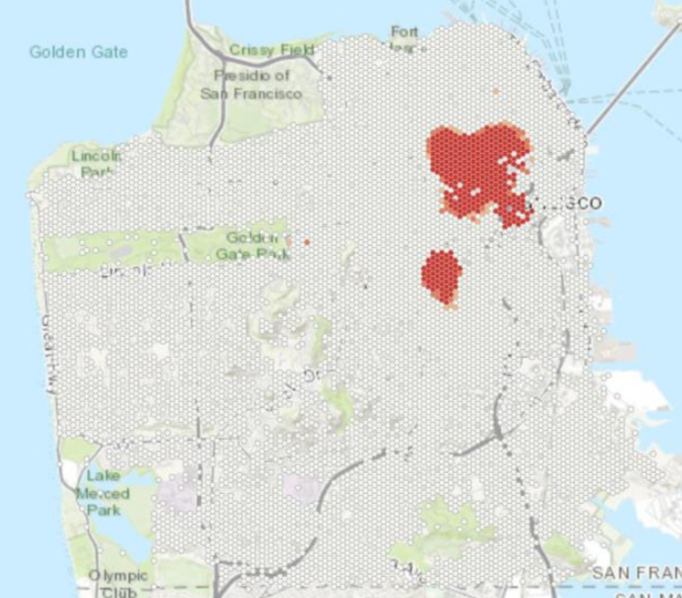
\includegraphics[width=8cm]{images_pfe/hotspot.png}
  \caption{Résultat d'une analyse de hotspot \parencite{kalinic_kernel_2018}.}
  \label{fig:vue-snoc-pos}
\end{figure}
\FloatBarrier

Lorem ipsum dolor sit amet, consectetur adipiscing elit. Proin posuere euismod neque, non semper nibh viverra sed. Praesent ut varius magna. Fusce ipsum ante, semper nec interdum at, semper et lacus. Nulla ultrices magna a fringilla finibus. Etiam sollicitudin blandit ante. Vivamus blandit rhoncus tincidunt. Morbi sit amet congue purus. Praesent interdum gravida congue. Donec fermentum dui fermentum maximus rutrum. \parencite{hart_kernel_2014,ansari_methods_2014,kalinic_kernel_2018}, Lorem ipsum dolor sit amet, consectetur adipiscing elit. Proin posuere euismod neque, non semper nibh viverra sed. Praesent ut varius magna. Fusce ipsum ante, semper nec interdum at, semper et lacus. Nulla ultrices magna a fringilla finibus. Etiam sollicitudin blandit ante. Vivamus blandit rhoncus tincidunt. Morbi sit amet congue purus. Praesent interdum gravida congue. Donec fermentum dui fermentum maximus rutrum. \parencite{anderson_kernel_2009,montella_comparative_2010,yu_comparative_2014}, Lorem ipsum dolor sit amet, consectetur adipiscing elit. Proin posuere euismod neque, non semper nibh viverra sed. Praesent ut varius magna. Fusce ipsum ante, semper nec interdum at, semper et lacus. Nulla ultrices magna a fringilla finibus. Etiam sollicitudin blandit ante. Vivamus blandit rhoncus tincidunt. Morbi sit amet congue purus. Praesent interdum gravida congue. Donec fermentum dui fermentum maximus rutrum. \parencite{lin_hotspot_2010}, Lorem ipsum dolor sit amet, consectetur adipiscing elit. Proin posuere euismod neque, non semper nibh viverra sed. Praesent ut varius magna. Fusce ipsum ante, semper nec interdum at, semper et lacus. Nulla ultrices magna a fringilla finibus. Etiam sollicitudin blandit ante. Vivamus blandit rhoncus tincidunt. Morbi sit amet congue purus. Praesent interdum gravida congue. Donec fermentum dui fermentum maximus rutrum. \parencite{bagstad_evaluating_2017}.

\subsection{Méthodes d'analyse des hotspots}

Lorem ipsum dolor sit amet, consectetur adipiscing elit. Proin posuere euismod neque, non semper nibh viverra sed. Praesent ut varius magna. Fusce ipsum ante, semper nec interdum at, semper et lacus. Nulla ultrices magna a fringilla finibus. Etiam sollicitudin blandit ante. Vivamus blandit rhoncus tincidunt. Morbi sit amet congue purus. Praesent interdum gravida congue. Donec fermentum dui fermentum maximus rutrum. \textbf{les méthodes d'interpolation spatiale} (Spatial Interpolation) et \textbf{les méthodes d'analyse de modèle spatial} (Pattern Analysis).

\medskip

Lorem ipsum dolor sit amet, consectetur adipiscing elit. Proin posuere euismod neque, non semper nibh viverra sed. Praesent ut varius magna. Fusce ipsum ante, semper nec interdum at, semper et lacus. Nulla ultrices magna a fringilla finibus. Etiam sollicitudin blandit ante. Vivamus blandit rhoncus tincidunt. Morbi sit amet congue purus. Praesent interdum gravida congue. Donec fermentum dui fermentum maximus rutrum. \parencite{chang_introduction_2019}. PLorem ipsum dolor sit amet, consectetur adipiscing elit. Proin posuere euismod neque, non semper nibh viverra sed. Praesent ut varius magna. Fusce ipsum ante, semper nec interdum at, semper et lacus. Nulla ultrices magna a fringilla finibus. Etiam sollicitudin blandit ante. Vivamus blandit rhoncus tincidunt. Morbi sit amet congue purus. Praesent interdum gravida congue. Donec fermentum dui fermentum maximus rutrum. \textbf{méthode d'estimation de la densité du noyau}.

\medskip

Lorem ipsum dolor sit amet, consectetur adipiscing elit. Proin posuere euismod neque, non semper nibh viverra sed. Praesent ut varius magna. Fusce ipsum ante, semper nec interdum at, semper et lacus. Nulla ultrices magna a fringilla finibus. Etiam sollicitudin blandit ante. Vivamus blandit rhoncus tincidunt. Morbi sit amet congue purus. Praesent interdum gravida congue. Donec fermentum dui fermentum maximus rutrum. \parencite{chang_introduction_2019}. Lorem ipsum dolor sit amet, consectetur adipiscing elit. Proin posuere euismod neque, non semper nibh viverra sed. Praesent ut varius magna. Fusce ipsum ante, semper nec interdum at, semper et lacus. Nulla ultrices magna a fringilla finibus. Etiam sollicitudin blandit ante. Vivamus blandit rhoncus tincidunt. Morbi sit amet congue purus. Praesent interdum gravida congue. Donec fermentum dui fermentum maximus rutrum. \textbf{statistique local de Moran} et la \textbf{statistique Gi* de Getis-Ord}.

\medskip

\subsubsection{Méthode d'estimation de la densité du noyeau (Kernel Density Estimation)}
Lorem ipsum dolor sit amet, consectetur adipiscing elit. Proin posuere euismod neque, non semper nibh viverra sed. Praesent ut varius magna. Fusce ipsum ante, semper nec interdum at, semper et lacus. Nulla ultrices magna a fringilla finibus. Etiam sollicitudin blandit ante. Vivamus blandit rhoncus tincidunt. Morbi sit amet congue purus. Praesent interdum gravida congue. Donec fermentum dui fermentum maximus rutrum. \parencite{hart_kernel_2014} (Voir figure \ref{fig:kde}).Lorem ipsum dolor sit amet, consectetur adipiscing elit. Proin posuere euismod neque, non semper nibh viverra sed. Praesent ut varius magna. Fusce ipsum ante, semper nec interdum at, semper et lacus. Nulla ultrices magna a fringilla finibus. Etiam sollicitudin blandit ante. Vivamus blandit rhoncus tincidunt. Morbi sit amet congue purus. Praesent interdum gravida congue. Donec fermentum dui fermentum maximus rutrum. \parencite{gatrell_spatial_1996}. 

\begin{figure}[hbt!]
  \centering
  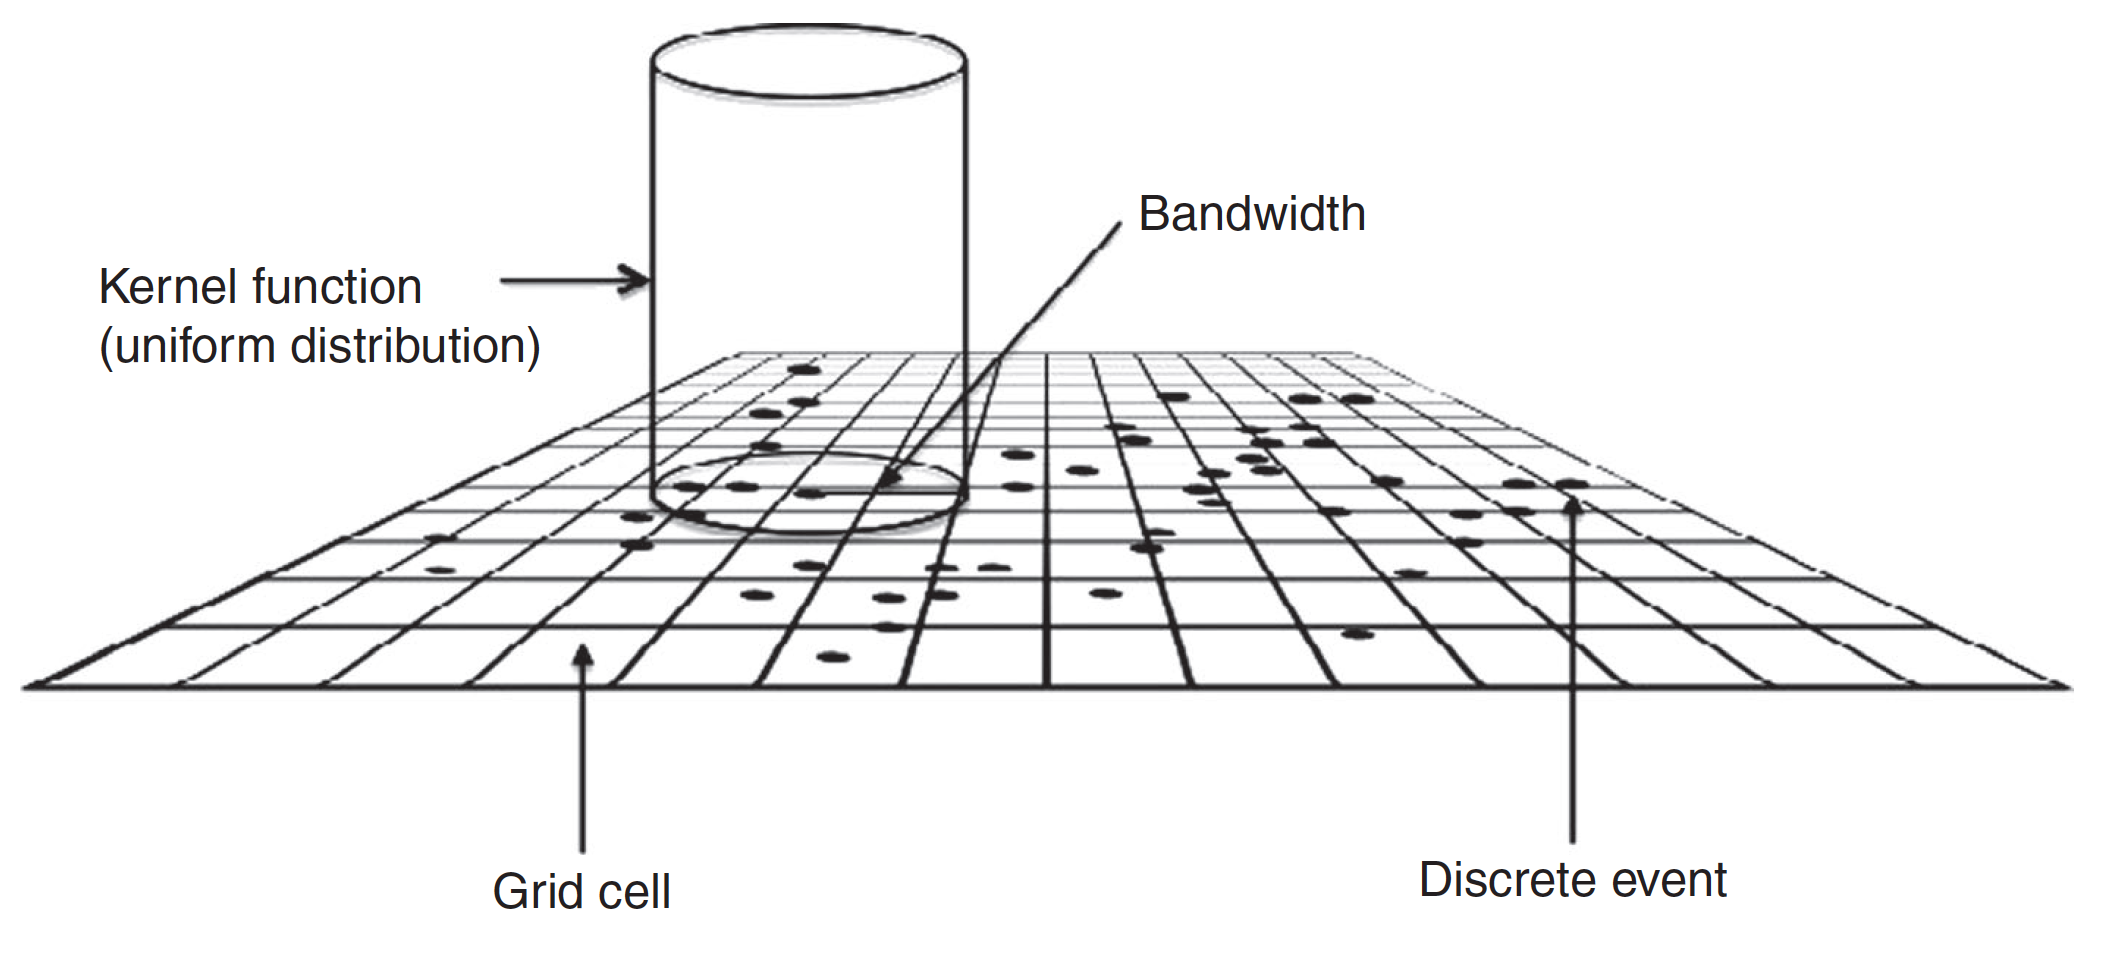
\includegraphics[width=14cm]{images_pfe/kernel_density_estimation.png}
  \caption{Estimation de la densité du noyau \parencite{hart_kernel_2014}}
  \label{fig:kde}
\end{figure}
\FloatBarrier

\medskip

\medskip

Lorem ipsum dolor sit amet, consectetur adipiscing elit. Proin posuere euismod neque, non semper nibh viverra sed. Praesent ut varius magna. Fusce ipsum ante, semper nec interdum at, semper et lacus. Nulla ultrices magna a fringilla finibus. Etiam sollicitudin blandit ante. Vivamus blandit rhoncus tincidunt. Morbi sit amet congue purus. Praesent interdum gravida congue. Donec fermentum dui fermentum maximus rutrum \parencite{fotheringham_quantitative_2007} :

\medskip

\begin{equation}
   \displaystyle f(x,y) = \frac{1}{nh} \sum_{i=1}^{n} K (\frac{d_i}{h})
   \label{kernel-density-estimation}
\end{equation}

\medskip

où $f(x, y)$ est l'estimation de la densité à l'emplacement $(x, y)$; $n$ est le nombre d'observations; $h$ est le rayon de recherche; $K$ est une fonction du noyau; et $d_i$ est la distance entre l'emplacement $(x, y)$ et l'emplacement de la $i$\up{ème} observation.




\medskip


\begin{figure}[hbt!]
  \centering
  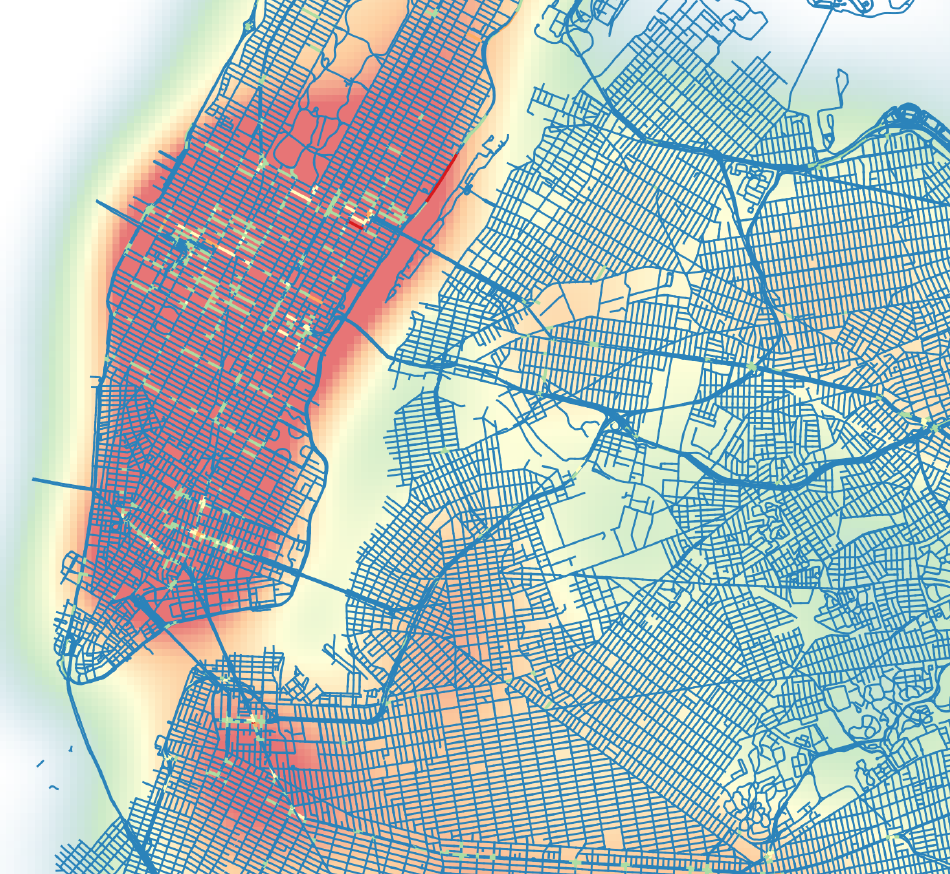
\includegraphics[width=10cm]{images_pfe/KDE_result.png}
  \caption{Exemple de résultat d'une analyse KDE \parencite{romano_visualizing_2017}}
  \label{fig:kde-result}
\end{figure}
\FloatBarrier

\medskip

\subsubsection{La statistique locale de Moran}
Lorem ipsum dolor sit amet, consectetur adipiscing elit. Proin posuere euismod neque, non semper nibh viverra sed. Praesent ut varius magna. Fusce ipsum ante, semper nec interdum at, semper et lacus. Nulla ultrices magna a fringilla finibus. Etiam sollicitudin blandit ante. Vivamus blandit rhoncus tincidunt. Morbi sit amet congue purus. Praesent interdum gravida congue. Donec fermentum dui fermentum maximus rutrum.\parencite{hart_kernel_2014}. 

\medskip

Lorem ipsum dolor sit amet, consectetur adipiscing elit. Proin posuere euismod neque, non semper nibh viverra sed. Praesent ut varius magna. Fusce ipsum ante, semper nec interdum at, semper et lacus. Nulla ultrices magna a fringilla finibus. Etiam sollicitudin blandit ante. Vivamus blandit rhoncus tincidunt. Morbi sit amet congue purus. Praesent interdum gravida congue. Donec fermentum dui fermentum maximus rutrum. \parencite{chang_introduction_2019}.

\medskip

Lorem ipsum dolor sit amet, consectetur adipiscing elit. Proin posuere euismod neque, non semper nibh viverra sed. Praesent ut varius magna. Fusce ipsum ante, semper nec interdum at, semper et lacus. Nulla ultrices magna a fringilla finibus. Etiam sollicitudin blandit ante. Vivamus blandit rhoncus tincidunt. Morbi sit amet congue purus. Praesent interdum gravida congue. Donec fermentum dui fermentum maximus rutrum. \parencite{hart_kernel_2014} :

\medskip

\begin{equation}
    I_i = \frac{x_i - \overline{X}}{ s_i^{2}} \sum_{j=1,j\neq i}^2 w_{ij}  (x_i - \overline{X})
\end{equation}

\medskip

où $x_i$ est un attribut pour l'entité $i$,  $\overline{X}$ est la moyenne de l'attribut correspondant, $w_{ij}$ est le poids spatial entre l'entité $i$ et $j$, et:

\medskip

\begin{equation}
    s_i^2 = \frac{\sum_{j=1,j\neq i}^2 w_{ij}  }{n-1} - \overline{X}^2
\end{equation}

\medskip
avec n égal au nombre total d'entités.
Le score $z_{I_{i}}$ pour les statistiques est calculé comme suit:
\medskip
\begin{equation}
    z_{I_{i}} = \frac{I_i - E [I_i]}{\sqrt{V[I_i]}}
\end{equation}

où:
\medskip

\begin{equation}
    E[I_i] = -\frac{\sum_{j=1,j\neq i}^2 w_{ij} }{n-1}
\end{equation}

\begin{equation}
    V[I_i] = E[I_i^2] - E[I_i]^2
\end{equation}

\medskip

\begin{figure}[hbt!]
  \centering
  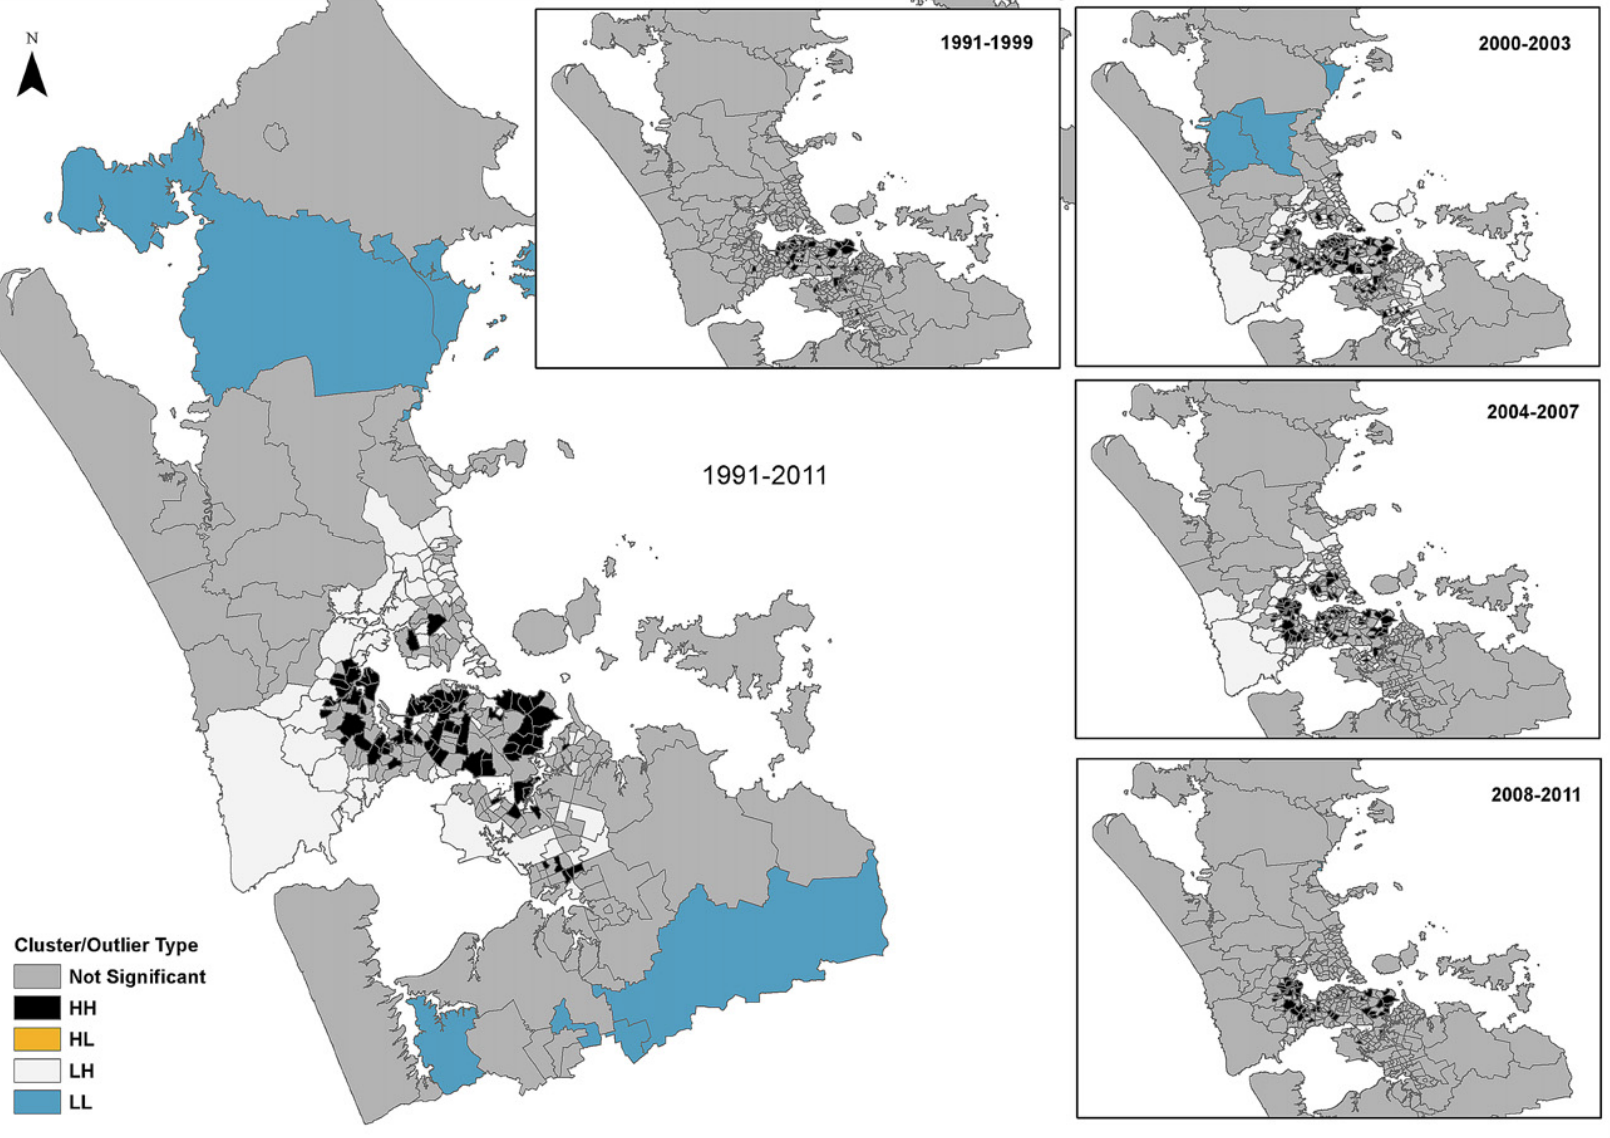
\includegraphics[width=10cm]{images_pfe/LSA_result.png}
  \caption{Résultat de l'analyse des points chauds avec la statistique locale de Moran \parencite{aguilar_distribution_2013}}
  \label{fig:lsa-result}
\end{figure}
\FloatBarrier

\medskip

\subsubsection{La statistique Gi*}
\label{subsec-gi-star}
Lorem ipsum dolor sit amet, consectetur adipiscing elit. Proin posuere euismod neque, non semper nibh viverra sed. Praesent ut varius magna. Fusce ipsum ante, semper nec interdum at, semper et lacus. Nulla ultrices magna a fringilla finibus. Etiam sollicitudin blandit ante. Vivamus blandit rhoncus tincidunt. Morbi sit amet congue purus. Praesent interdum gravida congue. Donec fermentum dui fermentum maximus rutrum. \parencite{getis_analysis_1992}. Lorem ipsum dolor sit amet, consectetur adipiscing elit. Proin posuere euismod neque, non semper nibh viverra sed. Praesent ut varius magna. Fusce ipsum ante, semper nec interdum at, semper et lacus. Nulla ultrices magna a fringilla finibus. Etiam sollicitudin blandit ante. Vivamus blandit rhoncus tincidunt. Morbi sit amet congue purus. Praesent interdum gravida congue. Donec fermentum dui fermentum maximus rutrum. \parencite{kalinic_kernel_2018}.Lorem ipsum dolor sit amet, consectetur adipiscing elit. Proin posuere euismod neque, non semper nibh viverra sed. Praesent ut varius magna. Fusce ipsum ante, semper nec interdum at, semper et lacus. Nulla ultrices magna a fringilla finibus. Etiam sollicitudin blandit ante. Vivamus blandit rhoncus tincidunt. Morbi sit amet congue purus. Praesent interdum gravida congue. Donec fermentum dui fermentum maximus rutrum. \parencite{getis_analysis_1992}. Lorem ipsum dolor sit amet, consectetur adipiscing elit. Proin posuere euismod neque, non semper nibh viverra sed. Praesent ut varius magna. Fusce ipsum ante, semper nec interdum at, semper et lacus. Nulla ultrices magna a fringilla finibus. Etiam sollicitudin blandit ante. Vivamus blandit rhoncus tincidunt. Morbi sit amet congue purus. Praesent interdum gravida congue. Donec fermentum dui fermentum maximus rutrum. \parencite{kalinic_kernel_2018}.
\medskip

La statistique Gi* est calculé comme suit \parencite{getis_analysis_1992}:

\medskip

\begin{equation}
    G_i^*(d) = \frac{\sum_{j=1}^n w_{ij}(d)x_j}{\sum_j x_j}
\end{equation}

\medskip
où $(w_{ij})$ est une matrice de poids spatial symétrique binaire avec des uns pour tous les liens définis comme étant à la distance $d$ d'un point $i$ donné, tous les autres liens sont nuls.
\medskip
Le score $Z_i$ est donné comme suit :
\medskip
\begin{equation}
    Z_i = \frac{G_i^*(d) - E [G_i^*(d)]}{\sqrt{V[G_i^*(d)]}}
\end{equation}

\medskip

où :

\medskip

\begin{equation}
    E[G_i^*(d)] = \frac{W_i^*}{n}
\end{equation}

\begin{equation}
    V[G_i^*(d)] = \frac{W_i^*(n - W_i^*)Y_{i2}^*}{n^2(n - 1) (Y_{i1}^*)^2}
\end{equation}

\medskip
avec :

\medskip
\begin{equation}
    W_i^* = \sum_{j=1}^n w_{ij}(d)
\end{equation}
\begin{equation}
    Y_{i1}^* = \frac{\sum_{j=1}^n x_j}{n}
\end{equation}

\begin{equation}
    Y_{i2}^* = \frac{\sum_{i=1}^n \sum_{j=1}^n (x_i x_j)^2}{n} - (Y_{i1}^*)^2
\end{equation}

\medskip

\begin{figure}[hbt!]
  \centering
  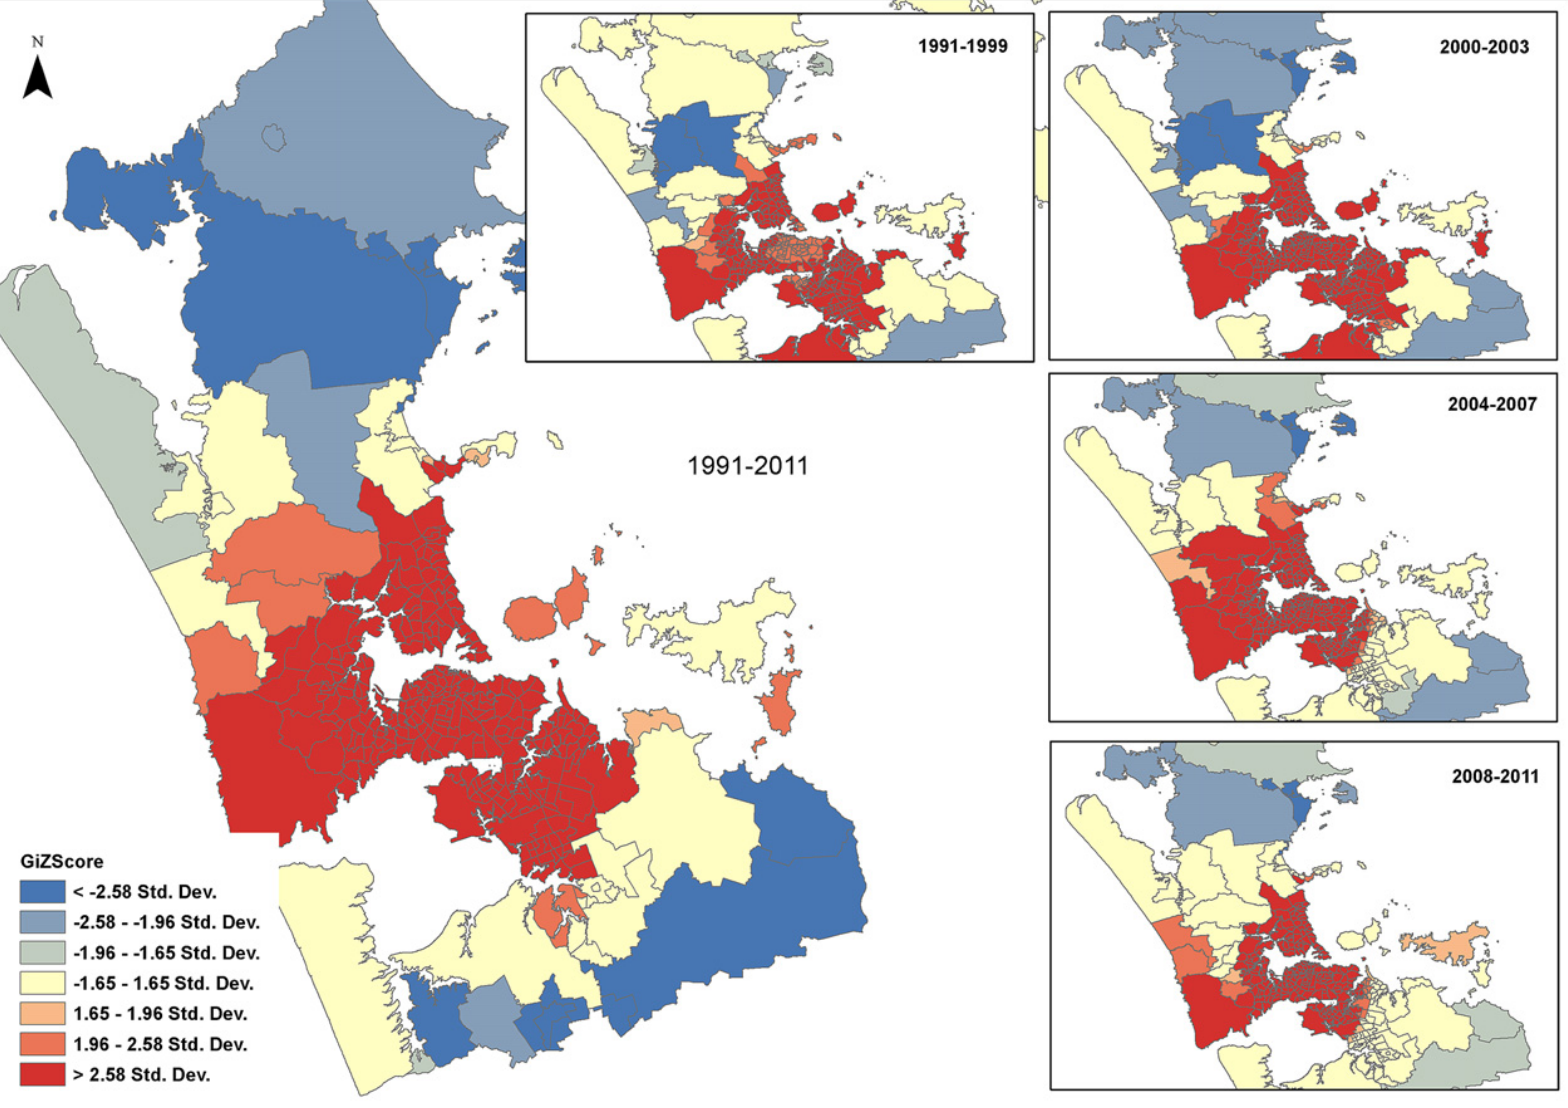
\includegraphics[width=10cm]{images_pfe/GI_result.png}
  \caption{Points chauds des colonies de chats sur la période 1991-2011 avec Gi* \parencite{aguilar_distribution_2013}}
  \label{fig:gi-result}
\end{figure}
\FloatBarrier

\medskip

\subsubsection{Comparaison entre les méthodes d'analyse des Hotspots}
Lorem ipsum dolor sit amet, consectetur adipiscing elit. Proin posuere euismod neque, non semper nibh viverra sed. Praesent ut varius magna. Fusce ipsum ante, semper nec interdum at, semper et lacus. Nulla ultrices magna a fringilla finibus. Etiam sollicitudin blandit ante. Vivamus blandit rhoncus tincidunt. Morbi sit amet congue purus. Praesent interdum gravida congue. Donec fermentum dui fermentum maximus rutrum.\parencite{kalinic_kernel_2018}.Lorem ipsum dolor sit amet, consectetur adipiscing elit. Proin posuere euismod neque, non semper nibh viverra sed. Praesent ut varius magna. Fusce ipsum ante, semper nec interdum at, semper et lacus. Nulla ultrices magna a fringilla finibus. Etiam sollicitudin blandit ante. Vivamus blandit rhoncus tincidunt. Morbi sit amet congue purus. Praesent interdum gravida congue. Donec fermentum dui fermentum maximus rutrum. \parencite{kalinic_kernel_2018}.

\medskip

Lorem ipsum dolor sit amet, consectetur adipiscing elit. Proin posuere euismod neque, non semper nibh viverra sed. Praesent ut varius magna. Fusce ipsum ante, semper nec interdum at, semper et lacus. Nulla ultrices magna a fringilla finibus. Etiam sollicitudin blandit ante. Vivamus blandit rhoncus tincidunt. Morbi sit amet congue purus. Praesent interdum gravida congue. Donec fermentum dui fermentum maximus rutrum.\parencite{chang_introduction_2019}. Lorem ipsum dolor sit amet, consectetur adipiscing elit. Proin posuere euismod neque, non semper nibh viverra sed. Praesent ut varius magna. Fusce ipsum ante, semper nec interdum at, semper et lacus. Nulla ultrices magna a fringilla finibus. Etiam sollicitudin blandit ante. Vivamus blandit rhoncus tincidunt. Morbi sit amet congue purus. Praesent interdum gravida congue. Donec fermentum dui fermentum maximus rutrum.

\medskip

Les tableaux \ref{tab:hotspot-analysis-comparison-1} et \ref{tab:hotspot-analysis-comparison-2} récapitulent les différences entre les trois méthodes :

\medskip

\begin{table}[h!]
    \centering
    \begin{tabular}{|c|c|c|}
        \hline
        Num & Méthode & Objectif \\
        \hline
         1 & KDE &  Pour un effet de lissage dans un certain rayon de recherche \\
        \hline
         2 & SLM & Pour détecter la présence de clusters de valeurs similaires \\
        \hline
        3 & Gi* &  Pour détecter la présence de clusters de valeurs faibles et élevées\\
        \hline
    \end{tabular}
    \caption{Les objectifs des trois méthodes d'analyse des hotspots}
    \label{tab:hotspot-analysis-comparison-1}
\end{table}
\FloatBarrier

\medskip

\begin{table}[h!]
    \centering
    \begin{tabular}{|c|c|c|c|c|c|c|}
        \hline
        \multirow{2}{*}{Num} & \multirow{2}{*}{Méthode} & \multicolumn{3}{c|}{Entité} &\multirow{2}{*}{Effet lissant} & \multirow{2}{*}{Z-score} \\
        \cline{3-5}
           & & Point & Ligne & Polygone & &  \\
        \hline
         1 & KDE & ++ & ++ & -- & ++ & --  \\
        \hline
         2 & SLM & ++ & -- & ++ & -- & ++  \\
        \hline
        3 & Gi* & ++ & --  & ++ & -- & ++ \\
        \hline
    \end{tabular}
    \caption{Comparaison entre les trois méthodes d'analyse des hotspots}
    \label{tab:hotspot-analysis-comparison-2}
\end{table}
\FloatBarrier




\section{Problème du voyageur de commerce (Traveling Salesman Problem)}
Lorem ipsum dolor sit amet, consectetur adipiscing elit. Proin posuere euismod neque, non semper nibh viverra sed. Praesent ut varius magna. Fusce ipsum ante, semper nec interdum at, semper et lacus. Nulla ultrices magna a fringilla finibus. Etiam sollicitudin blandit ante. Vivamus blandit rhoncus tincidunt. Morbi sit amet congue purus. Praesent interdum gravida congue. Donec fermentum dui fermentum maximus rutrum.


Lorem ipsum dolor sit amet, consectetur adipiscing elit. Proin posuere euismod neque, non semper nibh viverra sed. Praesent ut varius magna. Fusce ipsum ante, semper nec interdum at, semper et lacus. Nulla ultrices magna a fringilla finibus. Etiam sollicitudin blandit ante. Vivamus blandit rhoncus tincidunt. Morbi sit amet congue purus. Praesent interdum gravida congue. Donec fermentum dui fermentum maximus rutrum.. Les premières études du problème remontent au $18$\up{ème} siècle  avec les travaux d'Hamilton et Kirkman \parencite{davendra_traveling_2010}. Lorem ipsum dolor sit amet, consectetur adipiscing elit. Proin posuere euismod neque, non semper nibh viverra sed. Praesent ut varius magna. Fusce ipsum ante, semper nec interdum at, semper et lacus. Nulla ultrices magna a fringilla finibus. Etiam sollicitudin blandit ante. Vivamus blandit rhoncus tincidunt. Morbi sit amet congue purus. Praesent interdum gravida congue. Donec fermentum dui fermentum maximus rutrum. \parencite{gutin_traveling_2006}. Lorem ipsum dolor sit amet, consectetur adipiscing elit. Proin posuere euismod neque, non semper nibh viverra sed. Praesent ut varius magna. Fusce ipsum ante, semper nec interdum at, semper et lacus. Nulla ultrices magna a fringilla finibus. Etiam sollicitudin blandit ante. Vivamus blandit rhoncus tincidunt. Morbi sit amet congue purus. Praesent interdum gravida congue. Donec fermentum dui fermentum maximus rutrum.

\subsection{Formulation du problème}
Le problème dans sa forme générale peut être formulé comme suit :

\medskip
Soient $ V = \{v_1,...,v_n\} $ l'ensemble des villes (noeuds) à visiter, $ E = \{ (v_i,v_j) | v_i,v_j \in V \}$ l'ensemble des arcs entre les noeuds, $G = (V,E)$ un graphe complet et $C = (c_{ij})_{n × n}$ la matrice des coûts où $c_{ij}$ correspond au coût de l'arc reliant les noeuds $i$ et $j$ dans $G$. Le problème du voyageur de commerce est de trouver un tour (cycle hamiltonien) en $G$ tel que la somme des coûts des arcs du tour soit la plus petite possible.

\medskip

\begin{figure}[hbt!]
  \centering
  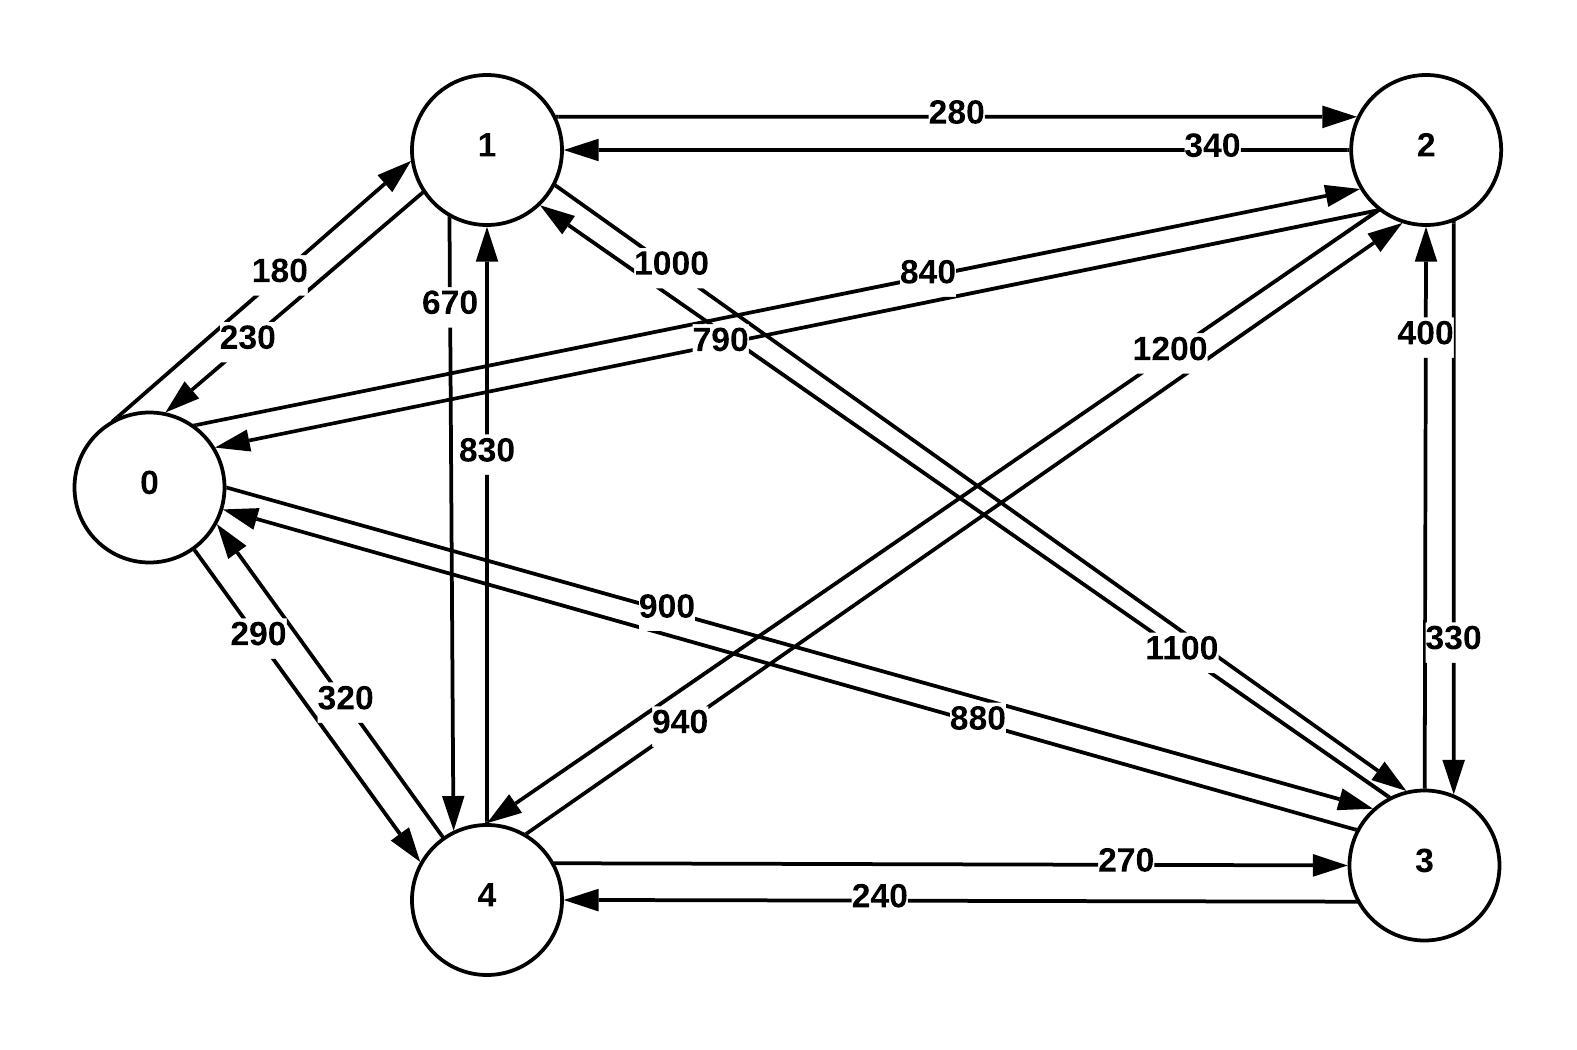
\includegraphics[width=12cm]{images_pfe/TSP_EXAMPLE.png}
  \caption{Exemple d'un TSP avec un point de départ et quatre noeuds. Les chiffres sur les arcs représentent les coûts.}
  \label{fig:tsp-example}
\end{figure}
\FloatBarrier

\subsection{Les approches de résolution du TSP}

Pour la résolution du TSP plusieurs approches ont été utilisées. Celles-ci peuvent être classées comme suit : approches exactes, approches heuristiques et approches métaheuristiques.

\medskip

\begin{figure}[hbt!]
  \centering
  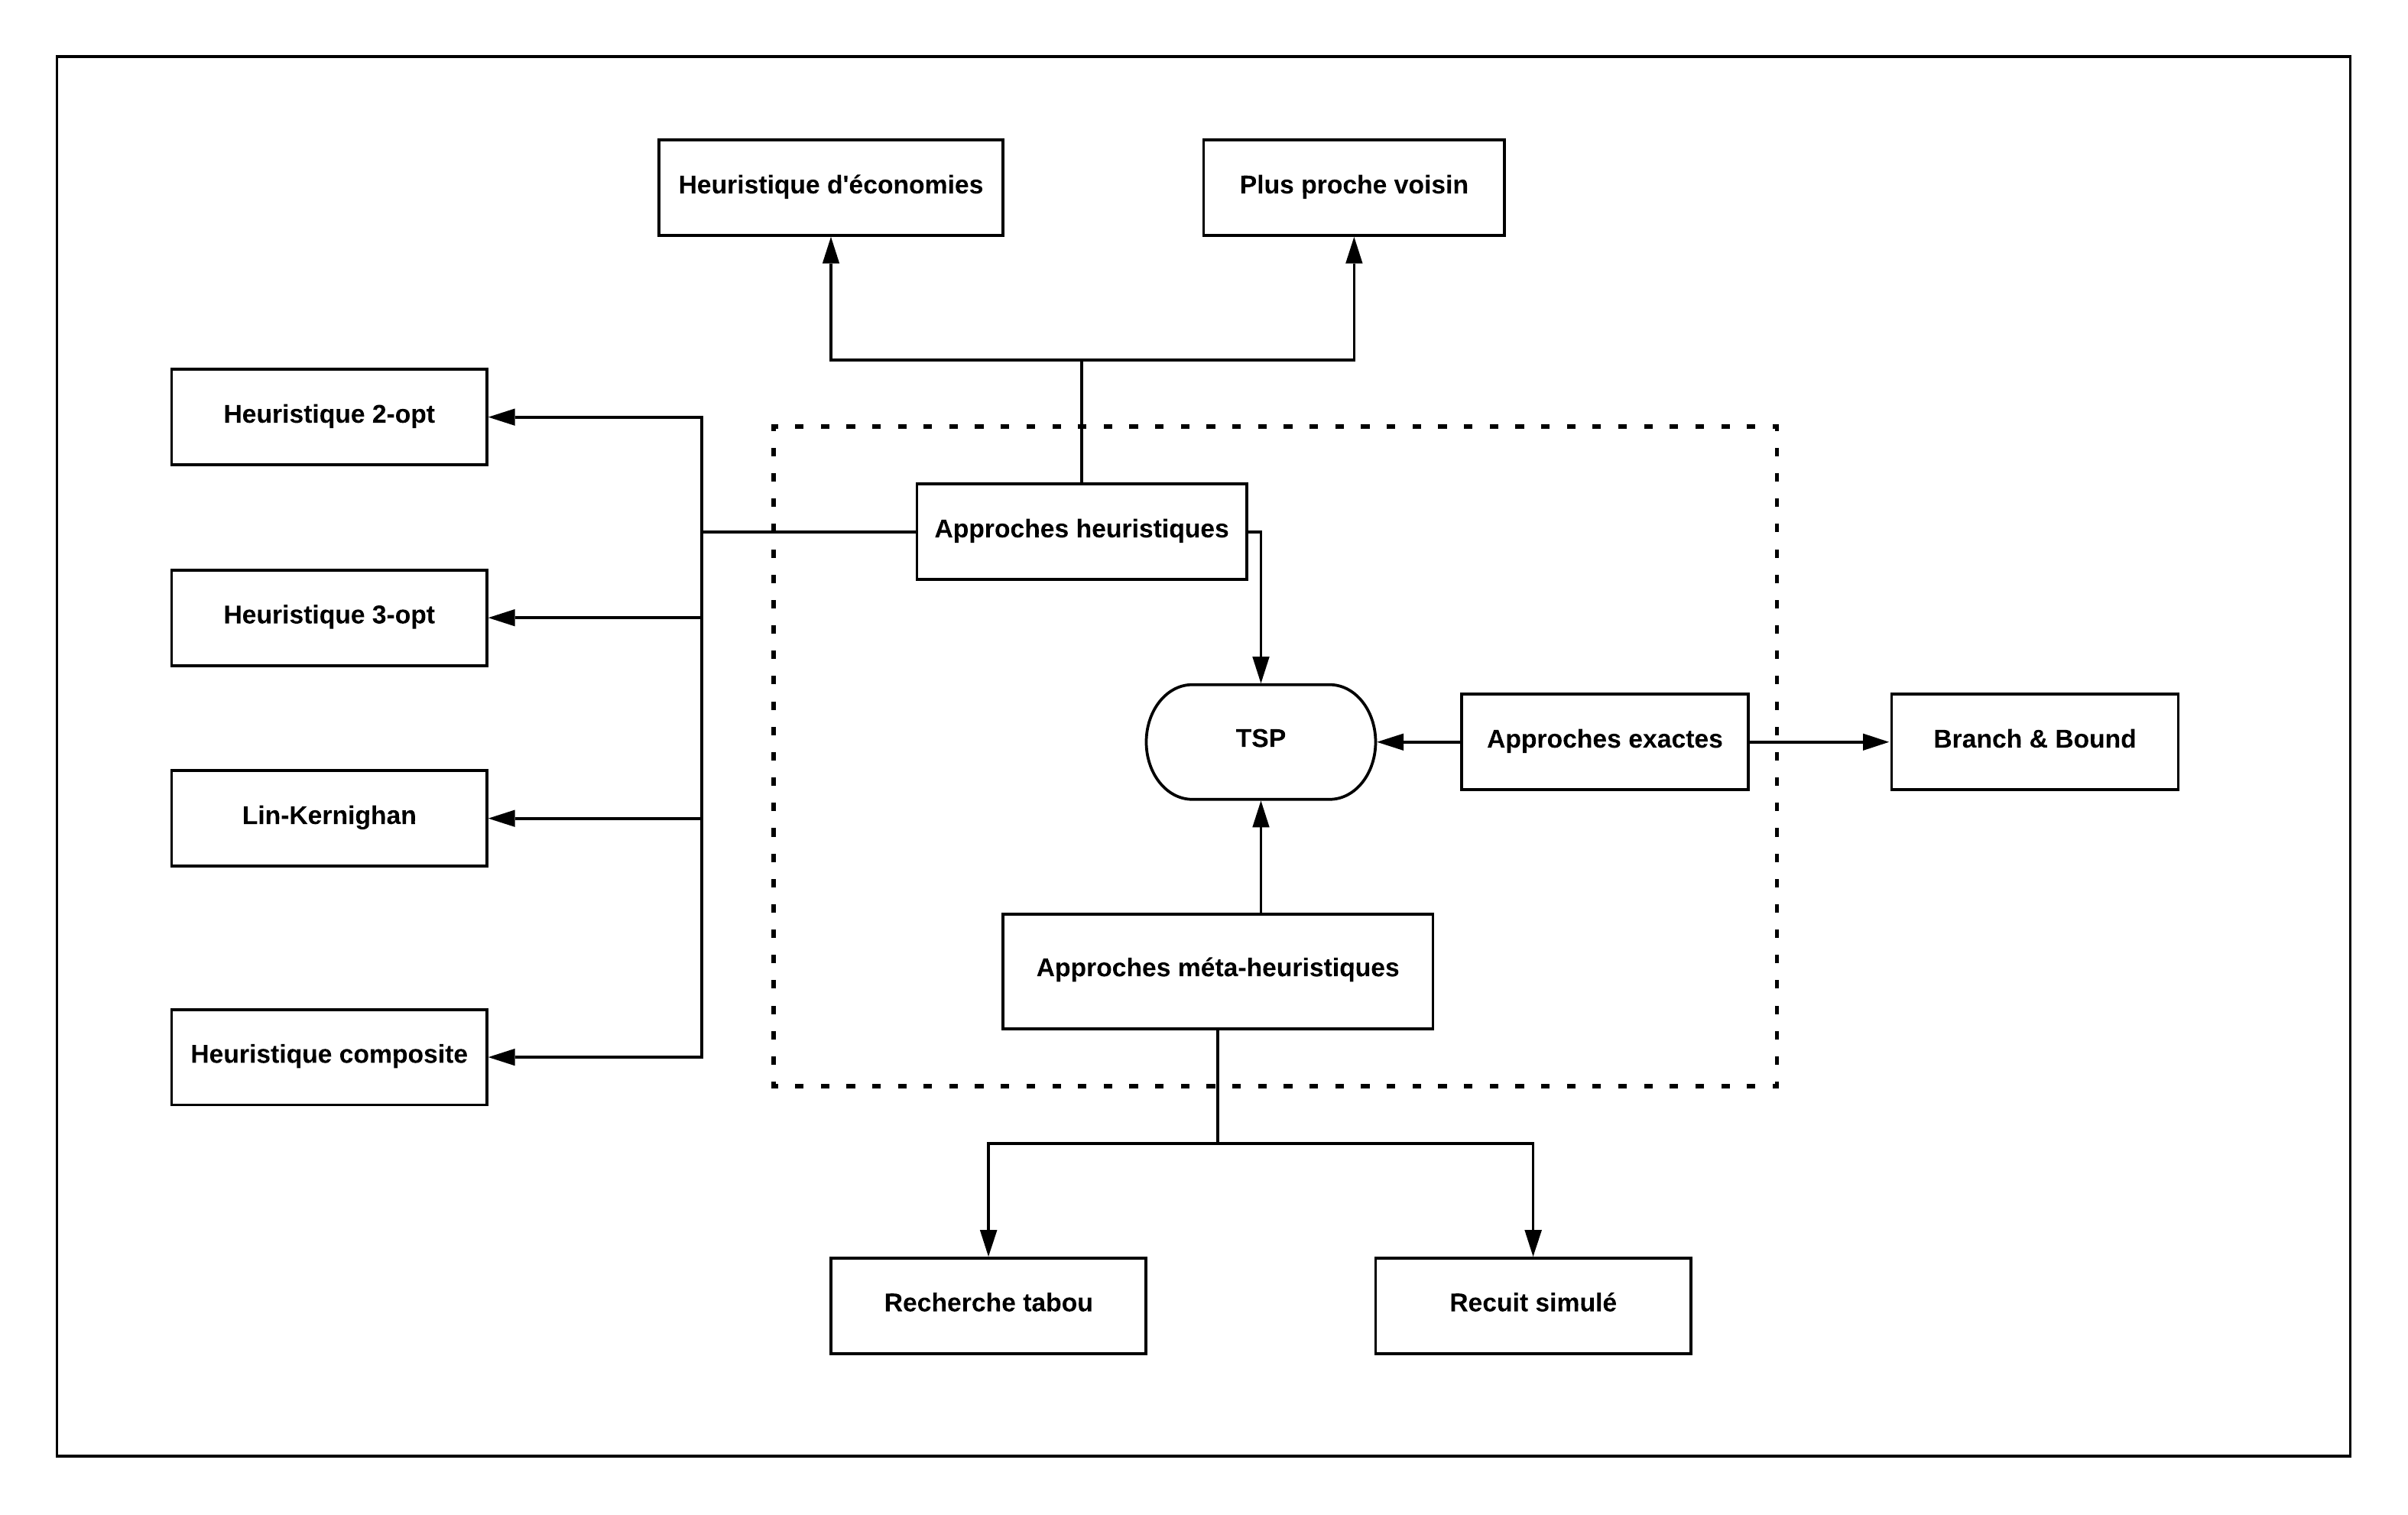
\includegraphics[width=15cm]{images_pfe/TSP_RESOLUTION_APPROCHES.png}
  \caption{Approches de résolution du TSP}
  \label{fig:tsp-solutions}
\end{figure}
\FloatBarrier

\medskip

\subsubsection{Approches exactes}
Lorem ipsum dolor sit amet, consectetur adipiscing elit. Proin posuere euismod neque, non semper nibh viverra sed. Praesent ut varius magna. Fusce ipsum ante, semper nec interdum at, semper et lacus. Nulla ultrices magna a fringilla finibus. Etiam sollicitudin blandit ante. Vivamus blandit rhoncus tincidunt. Morbi sit amet congue purus. Praesent interdum gravida congue. Donec fermentum dui fermentum maximus rutrum.. Parmi les solutions citées dans la littérature nous retrouvons l'algorithme Branch \& Bound \parencite{diderich_solving_1996,cotta_hybridizing_1995, tschoke_solving_1995}.

\medskip

\subsubsection{Approches heuristiques}
Lorem ipsum dolor sit amet, consectetur adipiscing elit. Proin posuere euismod neque, non semper nibh viverra sed. Praesent ut varius magna. Fusce ipsum ante, semper nec interdum at, semper et lacus. Nulla ultrices magna a fringilla finibus. Etiam sollicitudin blandit ante. Vivamus blandit rhoncus tincidunt. Morbi sit amet congue purus. Praesent interdum gravida congue. Donec fermentum dui fermentum maximus rutrum. \parencite{anbuudayasankar_survey_2014}.
Lorem ipsum dolor sit amet, consectetur adipiscing elit. Proin posuere euismod neque, non semper nibh viverra sed. Praesent ut varius magna. Fusce ipsum ante, semper nec interdum at, semper et lacus. Nulla ultrices magna a fringilla finibus. Etiam sollicitudin blandit ante. Vivamus blandit rhoncus tincidunt. Morbi sit amet congue purus. Praesent interdum gravida congue. Donec fermentum dui fermentum maximus rutrum.


\medskip

\subsubsection{Les heuristiques constructives}
Lorem ipsum dolor sit amet, consectetur adipiscing elit. Proin posuere euismod neque, non semper nibh viverra sed. Praesent ut varius magna. Fusce ipsum ante, semper nec interdum at, semper et lacus. Nulla ultrices magna a fringilla finibus. Etiam sollicitudin blandit ante. Vivamus blandit rhoncus tincidunt. Morbi sit amet congue purus. Praesent interdum gravida congue. Donec fermentum dui fermentum maximus rutrum. \parencite{anbuudayasankar_survey_2014}. Lorem ipsum dolor sit amet, consectetur adipiscing elit. Proin posuere euismod neque, non semper nibh viverra sed. Praesent ut varius magna. Fusce ipsum ante, semper nec interdum at, semper et lacus. Nulla ultrices magna a fringilla finibus. Etiam sollicitudin blandit ante. Vivamus blandit rhoncus tincidunt. Morbi sit amet congue purus. Praesent interdum gravida congue. Donec fermentum dui fermentum maximus rutrum.
\medskip

\paragraph{Plus proche voisin}
\label{par:nn}
Lorem ipsum dolor sit amet, consectetur adipiscing elit. Proin posuere euismod neque, non semper nibh viverra sed. Praesent ut varius magna. Fusce ipsum ante, semper nec interdum at, semper et lacus. Nulla ultrices magna a fringilla finibus. Etiam sollicitudin blandit ante. Vivamus blandit rhoncus tincidunt. Morbi sit amet congue purus. Praesent interdum gravida congue. Donec fermentum dui fermentum maximus rutrum. $O(n^2)$ \parencite{rosenkrantz_analysis_1977}.
Lorem ipsum dolor sit amet, consectetur adipiscing elit. Proin posuere euismod neque, non semper nibh viverra sed. Praesent ut varius magna. Fusce ipsum ante, semper nec interdum at, semper et lacus. Nulla ultrices magna a fringilla finibus. Etiam sollicitudin blandit ante. Vivamus blandit rhoncus tincidunt. Morbi sit amet congue purus. Praesent interdum gravida congue. Donec fermentum dui fermentum maximus rutrum. à moins de 25\% de la borne inférieure de Held-Karp (Voir \ref{held-karp}) \parencite{johnson_table_1995}.


\medskip


\paragraph{Heuristique d'économies}
Lorem ipsum dolor sit amet, consectetur adipiscing elit. Proin posuere euismod neque, non semper nibh viverra sed. Praesent ut varius magna. Fusce ipsum ante, semper nec interdum at, semper et lacus. Nulla ultrices magna a fringilla finibus. Etiam sollicitudin blandit ante. Vivamus blandit rhoncus tincidunt. Morbi sit amet congue purus. Praesent interdum gravida congue. Donec fermentum dui fermentum maximus rutrum. L'économie de la route reliant les noeuds $i$ et $j$ est donnée par $S_{ij} = c_{oi} + c_{oj} - c_{ij}$ tels que $c_{ij}$ est le coût entre les noeuds $i$ et $j$ et $c_{oi}$ est le coût entre le noeud de départ et le noeud $i$.Lorem ipsum dolor sit amet, consectetur adipiscing elit. Proin posuere euismod neque, non semper nibh viverra sed. Praesent ut varius magna. Fusce ipsum ante, semper nec interdum at, semper et lacus. Nulla ultrices magna a fringilla finibus. Etiam sollicitudin blandit ante. Vivamus blandit rhoncus tincidunt. Morbi sit amet congue purus. Praesent interdum gravida congue. Donec fermentum dui fermentum maximus rutrum. est égale à $O(n^2ln(n))$ \parencite{golden_approximate_1980}. 

\medskip

\subsubsection{Les heuristiques d'amélioration}
Lorem ipsum dolor sit amet, consectetur adipiscing elit. Proin posuere euismod neque, non semper nibh viverra sed. Praesent ut varius magna. Fusce ipsum ante, semper nec interdum at, semper et lacus. Nulla ultrices magna a fringilla finibus. Etiam sollicitudin blandit ante. Vivamus blandit rhoncus tincidunt. Morbi sit amet congue purus. Praesent interdum gravida congue. Donec fermentum dui fermentum maximus rutrum. \parencite{anbuudayasankar_survey_2014}. Lorem ipsum dolor sit amet, consectetur adipiscing elit. Proin posuere euismod neque, non semper nibh viverra sed. Praesent ut varius magna. Fusce ipsum ante, semper nec interdum at, semper et lacus. Nulla ultrices magna a fringilla finibus. Etiam sollicitudin blandit ante. Vivamus blandit rhoncus tincidunt. Morbi sit amet congue purus. Praesent interdum gravida congue. Donec fermentum dui fermentum maximus rutrum.


\paragraph{Les heuristiques 2-opt et 3-opt}
Lorem ipsum dolor sit amet, consectetur adipiscing elit. Proin posuere euismod neque, non semper nibh viverra sed. Praesent ut varius magna. Fusce ipsum ante, semper nec interdum at, semper et lacus. Nulla ultrices magna a fringilla finibus. Etiam sollicitudin blandit ante. Vivamus blandit rhoncus tincidunt. Morbi sit amet congue purus. Praesent interdum gravida congue. Donec fermentum dui fermentum maximus rutrum. (Voir figure \ref{fig:two-opt}). Lorem ipsum dolor sit amet, consectetur adipiscing elit. Proin posuere euismod neque, non semper nibh viverra sed. Praesent ut varius magna. Fusce ipsum ante, semper nec interdum at, semper et lacus. Nulla ultrices magna a fringilla finibus. Etiam sollicitudin blandit ante. Vivamus blandit rhoncus tincidunt. Morbi sit amet congue purus. Praesent interdum gravida congue. Donec fermentum dui fermentum maximus rutrum. (Voir figure \ref{fig:three-opt}).Lorem ipsum dolor sit amet, consectetur adipiscing elit. Proin posuere euismod neque, non semper nibh viverra sed. Praesent ut varius magna. Fusce ipsum ante, semper nec interdum at, semper et lacus. Nulla ultrices magna a fringilla finibus. Etiam sollicitudin blandit ante. Vivamus blandit rhoncus tincidunt. Morbi sit amet congue purus. Praesent interdum gravida congue. Donec fermentum dui fermentum maximus rutrump \parencite{davendra_traveling_2010}. La complexité d'une heuristique k-opt est égale à $O(n^k)$ \parencite{golden_approximate_1980}.

\begin{figure}[hbt!]
  \centering
  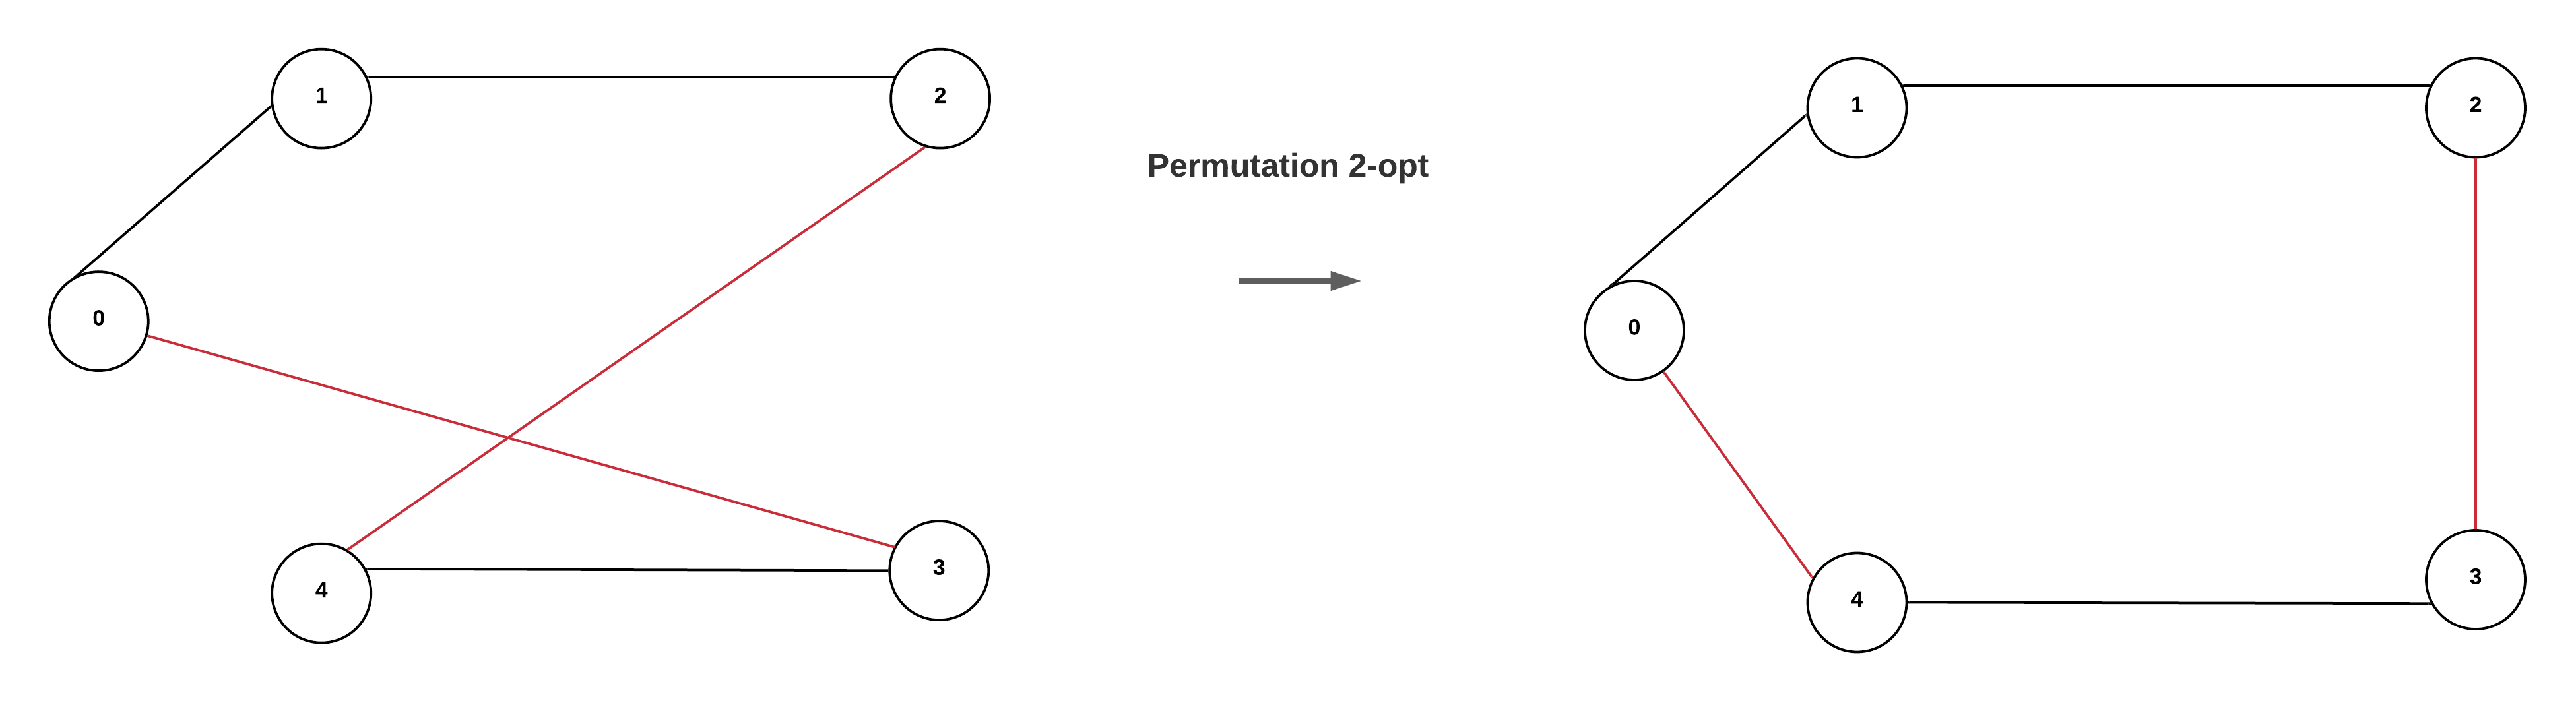
\includegraphics[width=15cm]{images_pfe/TWO_OPT.png}
  \caption{Permutation 2-opt.}
  \label{fig:two-opt}
\end{figure}
\FloatBarrier

\begin{figure}[hbt!]
  \centering
  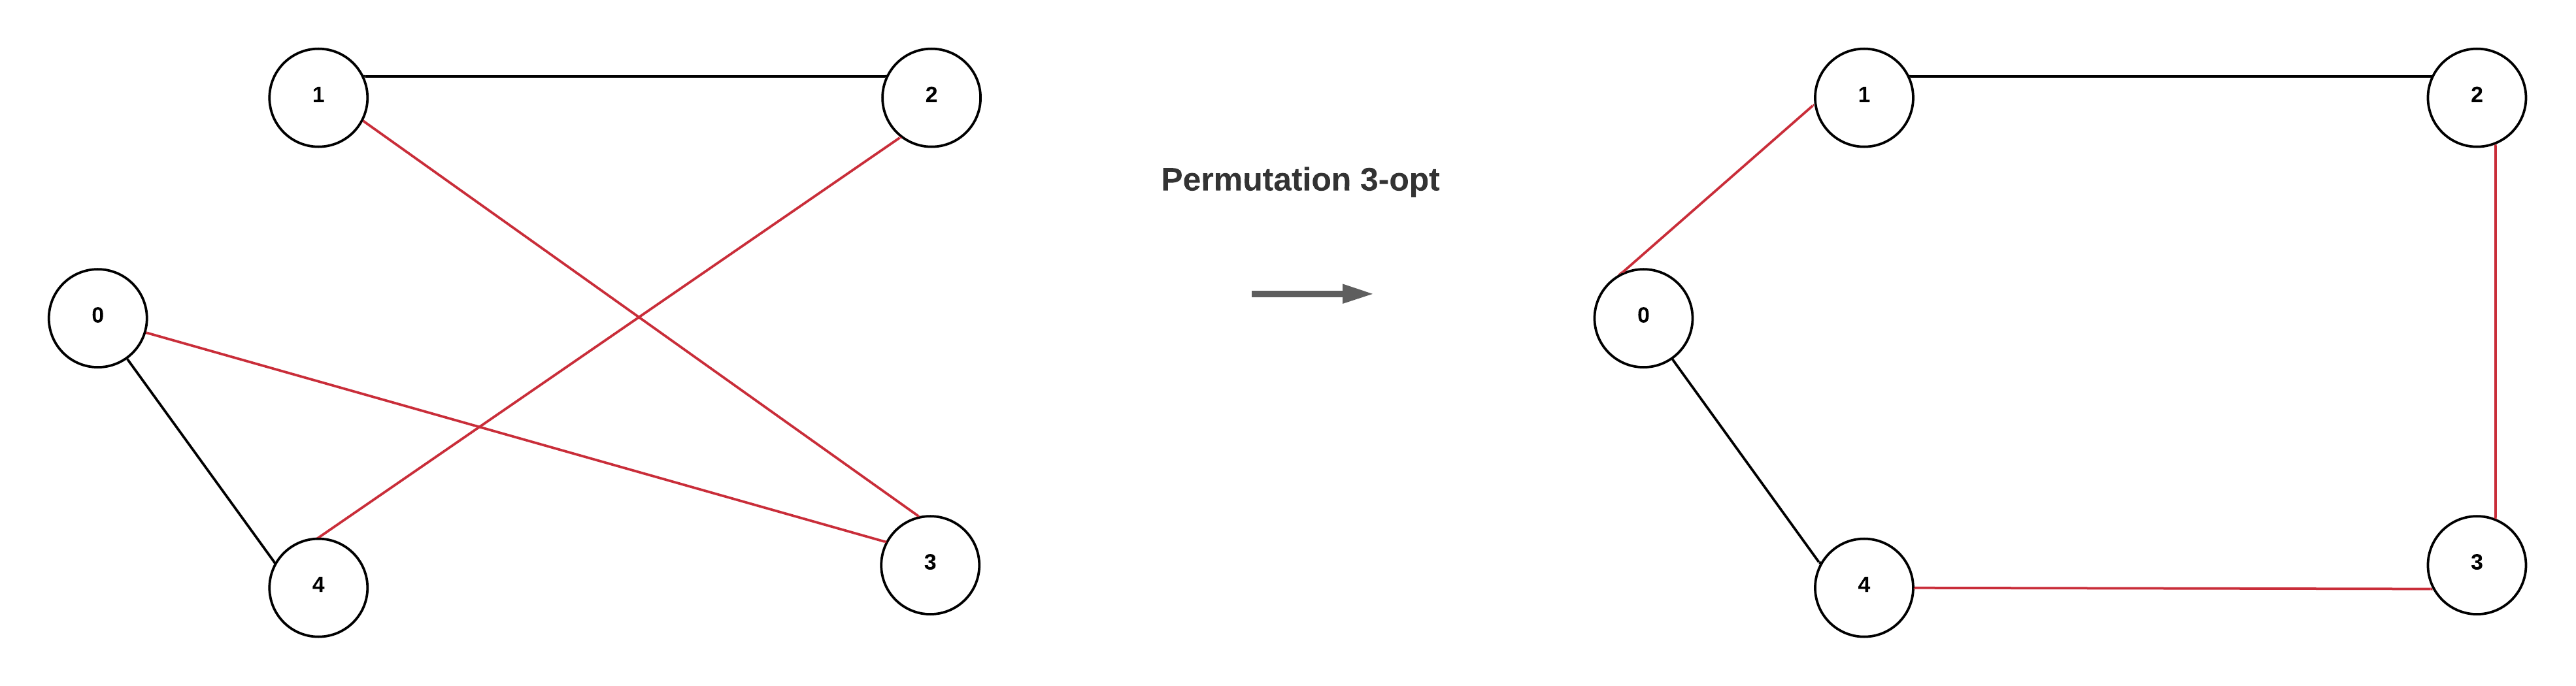
\includegraphics[width=15cm]{images_pfe/THREE_OPT.png}
  \caption{Permutation 3-opt.}
  \label{fig:three-opt}
\end{figure}
\FloatBarrier


\medskip

\paragraph{Heuristique Lin-Kernighan}
\label{par:lin-kernighan}
Lorem ipsum dolor sit amet, consectetur adipiscing elit. Proin posuere euismod neque, non semper nibh viverra sed. Praesent ut varius magna. Fusce ipsum ante, semper nec interdum at, semper et lacus. Nulla ultrices magna a fringilla finibus. Etiam sollicitudin blandit ante. Vivamus blandit rhoncus tincidunt. Morbi sit amet congue purus. Praesent interdum gravida congue. Donec fermentum dui fermentum maximus rutrum. La complexité temporelle de LK est d'environ $O(n^{2.2})$ \parencite{helsgaun_effective_2000}.

\medskip

\paragraph{La borne inférieure de Held-Karp }
\label{held-karp}
Lorem ipsum dolor sit amet, consectetur adipiscing elit. Proin posuere euismod neque, non semper nibh viverra sed. Praesent ut varius magna. Fusce ipsum ante, semper nec interdum at, semper et lacus. Nulla ultrices magna a fringilla finibus. Etiam sollicitudin blandit ante. Vivamus blandit rhoncus tincidunt. Morbi sit amet congue purus. Praesent interdum gravida congue. Donec fermentum dui fermentum maximus rutrum.Une borne inférieure Held-Karp est en moyenne d'environ 0,8\% inférieure à la durée optimale du tour \parencite{johnson_asymptotic_1996}.

\medskip

\subsubsection{Les heuristiques composites}
Lorem ipsum dolor sit amet, consectetur adipiscing elit. Proin posuere euismod neque, non semper nibh viverra sed. Praesent ut varius magna. Fusce ipsum ante, semper nec interdum at, semper et lacus. Nulla ultrices magna a fringilla finibus. Etiam sollicitudin blandit ante. Vivamus blandit rhoncus tincidunt. Morbi sit amet congue purus. Praesent interdum gravida congue. Donec fermentum dui fermentum maximus rutrum. \parencite{golden_approximate_1980}.

\subsubsection{Les approches métaheuristiques}
Lorem ipsum dolor sit amet, consectetur adipiscing elit. Proin posuere euismod neque, non semper nibh viverra sed. Praesent ut varius magna. Fusce ipsum ante, semper nec interdum at, semper et lacus. Nulla ultrices magna a fringilla finibus. Etiam sollicitudin blandit ante. Vivamus blandit rhoncus tincidunt. Morbi sit amet congue purus. Praesent interdum gravida congue. Donec fermentum dui fermentum maximus rutrum.\parencite{blum_metaheuristics_2003}. Lorem ipsum dolor sit amet, consectetur adipiscing elit. Proin posuere euismod neque, non semper nibh viverra sed. Praesent ut varius magna. Fusce ipsum ante, semper nec interdum at, semper et lacus. Nulla ultrices magna a fringilla finibus. Etiam sollicitudin blandit ante. Vivamus blandit rhoncus tincidunt. Morbi sit amet congue purus. Praesent interdum gravida congue. Donec fermentum dui fermentum maximus rutrum. \parencite{bianchi_survey_2009}.

\medskip

\paragraph{Recherche tabou}
Lorem ipsum dolor sit amet, consectetur adipiscing elit. Proin posuere euismod neque, non semper nibh viverra sed. Praesent ut varius magna. Fusce ipsum ante, semper nec interdum at, semper et lacus. Nulla ultrices magna a fringilla finibus. Etiam sollicitudin blandit ante. Vivamus blandit rhoncus tincidunt. Morbi sit amet congue purus. Praesent interdum gravida congue. Donec fermentum dui fermentum maximus rutrum. $O(n^3)$, ce qui la rend beaucoup plus lente qu'une recherche locale à 2 permutations \parencite{davendra_traveling_2010}.

\medskip

\paragraph{Recuit simulé}
Lorem ipsum dolor sit amet, consectetur adipiscing elit. Proin posuere euismod neque, non semper nibh viverra sed. Praesent ut varius magna. Fusce ipsum ante, semper nec interdum at, semper et lacus. Nulla ultrices magna a fringilla finibus. Etiam sollicitudin blandit ante. Vivamus blandit rhoncus tincidunt. Morbi sit amet congue purus. Praesent interdum gravida congue. Donec fermentum dui fermentum maximus rutrum. \parencite{johnson_traveling_1995} Lorem ipsum dolor sit amet, consectetur adipiscing elit. Proin posuere euismod neque, non semper nibh viverra sed. Praesent ut varius magna. Fusce ipsum ante, semper nec interdum at, semper et lacus. Nulla ultrices magna a fringilla finibus. Etiam sollicitudin blandit ante. Vivamus blandit rhoncus tincidunt. Morbi sit amet congue purus. Praesent interdum gravida congue. Donec fermentum dui fermentum maximus rutrum. En raison du voisinage à 2-opt, cette implémentation particulière prend $O(n^2)$ avec une grande constante de proportionnalité \parencite{davendra_traveling_2010}.

\medskip

\section{Problème du voyageur de commerce avec contrainte périodique (Periodic Traveling Salesman Problem)}
\label{sec:ptsp}
Lorem ipsum dolor sit amet, consectetur adipiscing elit. Proin posuere euismod neque, non semper nibh viverra sed. Praesent ut varius magna. Fusce ipsum ante, semper nec interdum at, semper et lacus. Nulla ultrices magna a fringilla finibus. Etiam sollicitudin blandit ante. Vivamus blandit rhoncus tincidunt. Morbi sit amet congue purus. Praesent interdum gravida congue. Donec fermentum dui fermentum maximus rutrum. \parencite{paletta_period_2002}. Lorem ipsum dolor sit amet, consectetur adipiscing elit. Proin posuere euismod neque, non semper nibh viverra sed. Praesent ut varius magna. Fusce ipsum ante, semper nec interdum at, semper et lacus. Nulla ultrices magna a fringilla finibus. Etiam sollicitudin blandit ante. Vivamus blandit rhoncus tincidunt. Morbi sit amet congue purus. Praesent interdum gravida congue. Donec fermentum dui fermentum maximus rutrum. \parencite{cordeau_tabu_1997}Lorem ipsum dolor sit amet, consectetur adipiscing elit. Proin posuere euismod neque, non semper nibh viverra sed. Praesent ut varius magna. Fusce ipsum ante, semper nec interdum at, semper et lacus. Nulla ultrices magna a fringilla finibus. Etiam sollicitudin blandit ante. Vivamus blandit rhoncus tincidunt. Morbi sit amet congue purus. Praesent interdum gravida congue. Donec fermentum dui fermentum maximus rutrum.

\medskip

\subsection{Formulation du problème}
Le PTSP peut être formulé comme un problème d'optimisation combinatoire. Soit $V$ l'ensemble des points client, y compris la ville d'origine. Soit $E$ l'ensemble des arcs entre chaque paire de points dans $V$ et que chaque arc dans $E$ ait un poids non négatif $c_{ij}$ qui lui est associée, où $c_{ij}$ est la distance entre le point $i$ et le point $j$. Alors $G = (V, E)$ est un graphe complet et nous devons construire $M$ cycles afin que chaque point client en $V$ soit visité le nombre de fois requis pendant la période de $M$ jours et le coût total du voyage sur toute la période est minimisé \parencite{chao_new_1995}.


\begin{figure}[hbt!]
  \centering
  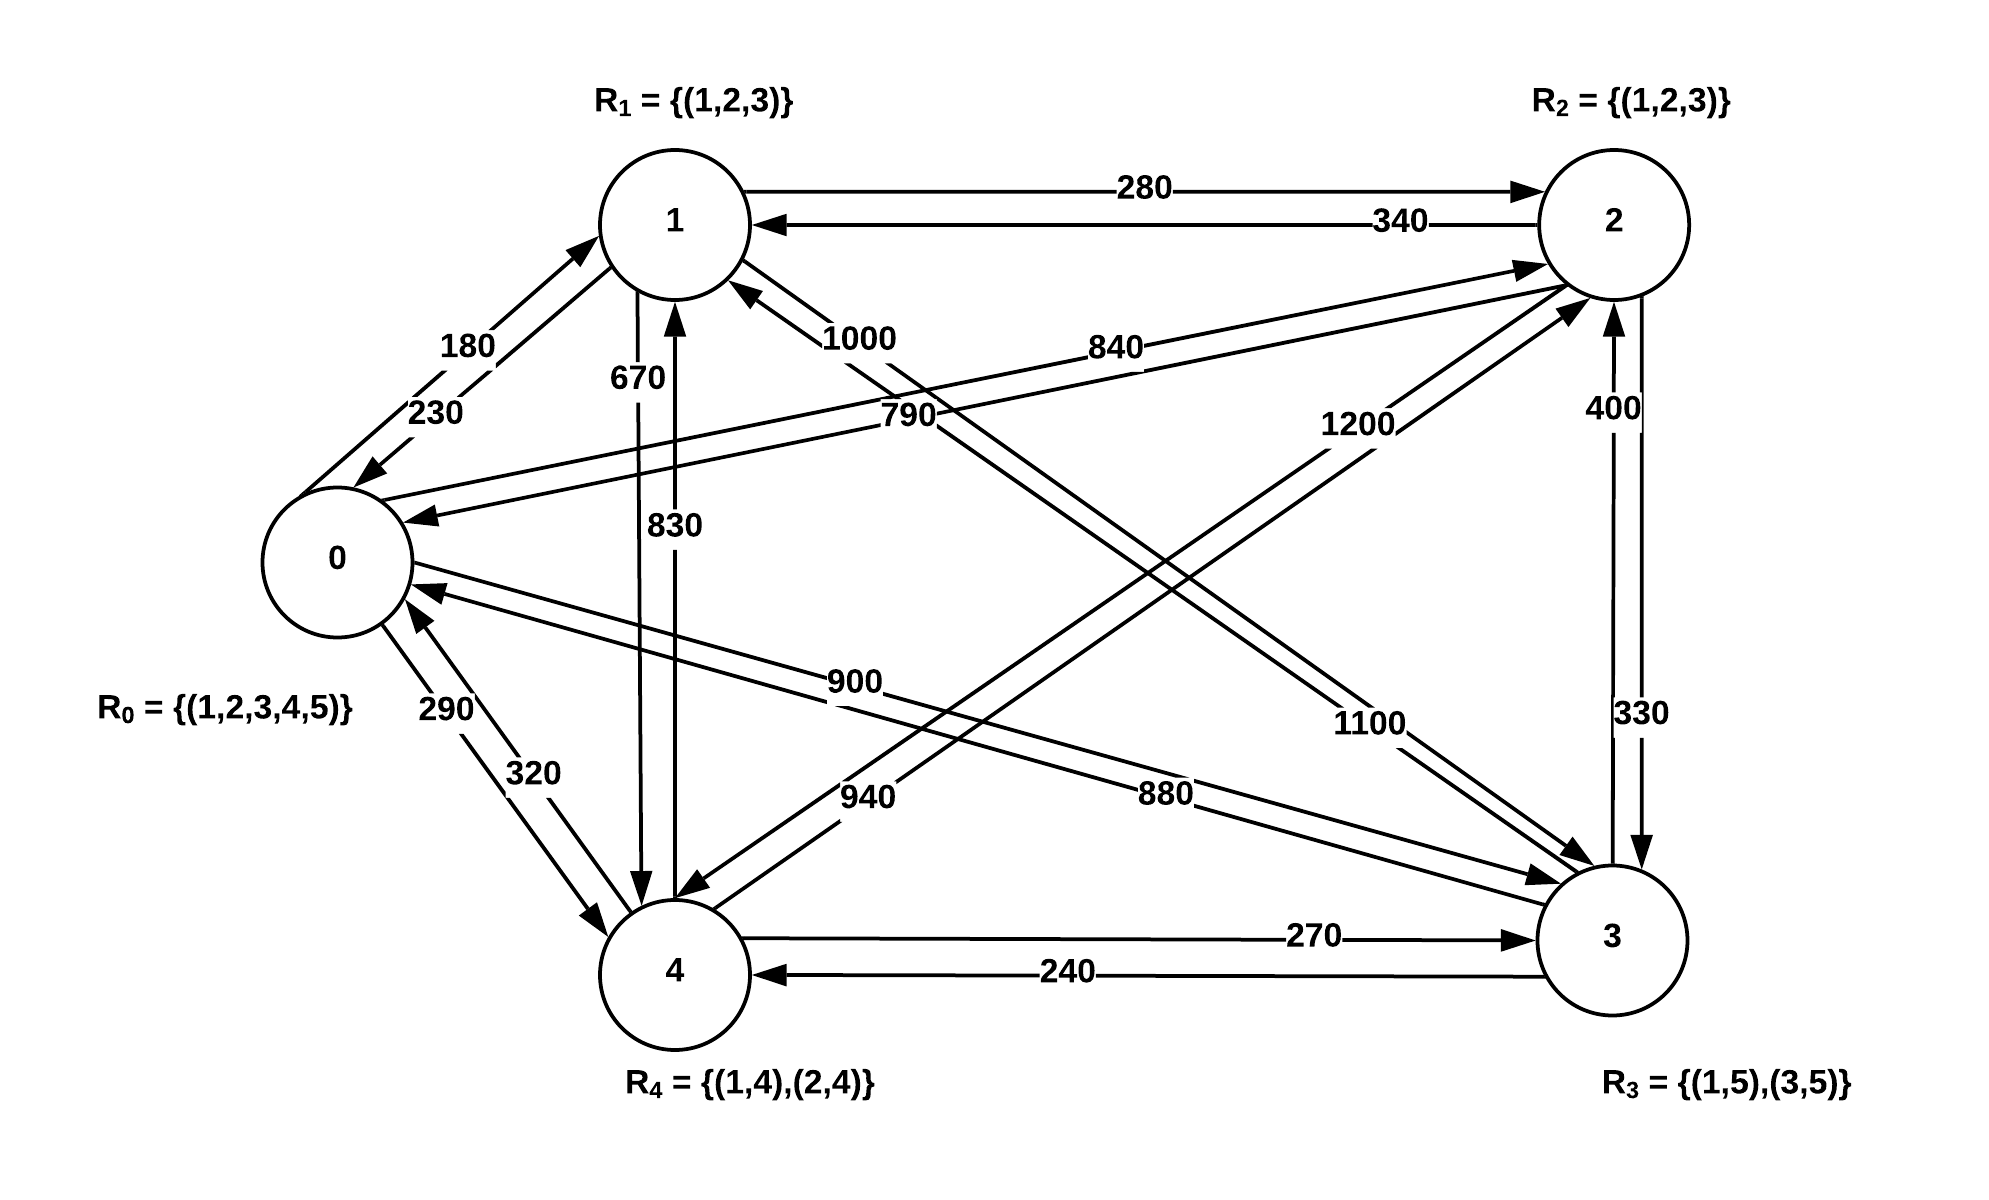
\includegraphics[height=10cm]{images_pfe/PTSP_EXAMPLE.png}
  \caption{Exemple d'un PTSP avec un point de départ et quatre noeuds sur une période de 5 jours. Les $R_i$ représentent les combinaisons de visites et les chiffres sur les arcs représentent les coûts (distances de parcours). Exemple : le noeud 4 peut être visité soit les jours 1 et 4 ou les jours 2 et 4. }
  \label{fig:ptsp-first-example}
\end{figure}
\FloatBarrier



\subsection{Les approches de résolution du PTSP}
Lorem ipsum dolor sit amet, consectetur adipiscing elit. Proin posuere euismod neque, non semper nibh viverra sed. Praesent ut varius magna. Fusce ipsum ante, semper nec interdum at, semper et lacus. Nulla ultrices magna a fringilla finibus. Etiam sollicitudin blandit ante. Vivamus blandit rhoncus tincidunt. Morbi sit amet congue purus. Praesent interdum gravida congue. Donec fermentum dui fermentum maximus rutrum.

\medskip

\subsubsection{L'heuristique CGW de \parencite{chao_new_1995}}
Lorem ipsum dolor sit amet, consectetur adipiscing elit. Proin posuere euismod neque, non semper nibh viverra sed. Praesent ut varius magna. Fusce ipsum ante, semper nec interdum at, semper et lacus. Nulla ultrices magna a fringilla finibus. Etiam sollicitudin blandit ante. Vivamus blandit rhoncus tincidunt. Morbi sit amet congue purus. Praesent interdum gravida congue. Donec fermentum dui fermentum maximus rutrum. Lorem ipsum dolor sit amet, consectetur adipiscing elit. Proin posuere euismod neque, non semper nibh viverra sed. Praesent ut varius magna. Fusce ipsum ante, semper nec interdum at, semper et lacus. Nulla ultrices magna a fringilla finibus. Etiam sollicitudin blandit ante. Vivamus blandit rhoncus tincidunt. Morbi sit amet congue purus. Praesent interdum gravida congue. Donec fermentum dui fermentum maximus rutrum.

\subsubsection{La recherche tabou CGL de \parencite{cordeau_tabu_1997} }
Lorem ipsum dolor sit amet, consectetur adipiscing elit. Proin posuere euismod neque, non semper nibh viverra sed. Praesent ut varius magna. Fusce ipsum ante, semper nec interdum at, semper et lacus. Nulla ultrices magna a fringilla finibus. Etiam sollicitudin blandit ante. Vivamus blandit rhoncus tincidunt. Morbi sit amet congue purus. Praesent interdum gravida congue. Donec fermentum dui fermentum maximus rutrum.

\medskip

\subsubsection{L'heuristique P de \parencite{paletta_period_2002}}
Lorem ipsum dolor sit amet, consectetur adipiscing elit. Proin posuere euismod neque, non semper nibh viverra sed. Praesent ut varius magna. Fusce ipsum ante, semper nec interdum at, semper et lacus. Nulla ultrices magna a fringilla finibus. Etiam sollicitudin blandit ante. Vivamus blandit rhoncus tincidunt. Morbi sit amet congue purus. Praesent interdum gravida congue. Donec fermentum dui fermentum maximus rutrum.

\medskip

\subsubsection{L'heuristique BPS de \parencite{bertazzi_improved_2004}}
Lorem ipsum dolor sit amet, consectetur adipiscing elit. Proin posuere euismod neque, non semper nibh viverra sed. Praesent ut varius magna. Fusce ipsum ante, semper nec interdum at, semper et lacus. Nulla ultrices magna a fringilla finibus. Etiam sollicitudin blandit ante. Vivamus blandit rhoncus tincidunt. Morbi sit amet congue purus. Praesent interdum gravida congue. Donec fermentum dui fermentum maximus rutrum. \parencite{paletta_period_2002}. Lorem ipsum dolor sit amet, consectetur adipiscing elit. Proin posuere euismod neque, non semper nibh viverra sed. Praesent ut varius magna. Fusce ipsum ante, semper nec interdum at, semper et lacus. Nulla ultrices magna a fringilla finibus. Etiam sollicitudin blandit ante. Vivamus blandit rhoncus tincidunt. Morbi sit amet congue purus. Praesent interdum gravida congue. Donec fermentum dui fermentum maximus rutrum.

\medskip

\subsubsection{La métaheuristique HDH de \parencite{hemmelmayr_variable_2009}}
\label{sub-sec:hdh}
Lorem ipsum dolor sit amet, consectetur adipiscing elit. Proin posuere euismod neque, non semper nibh viverra sed. Praesent ut varius magna. Fusce ipsum ante, semper nec interdum at, semper et lacus. Nulla ultrices magna a fringilla finibus. Etiam sollicitudin blandit ante. Vivamus blandit rhoncus tincidunt. Morbi sit amet congue purus. Praesent interdum gravida congue. Donec fermentum dui fermentum maximus rutrum.
\medskip

\subsubsection{L'heuristique IPH de \parencite{gulczynski_period_2011}}
Lorem ipsum dolor sit amet, consectetur adipiscing elit. Proin posuere euismod neque, non semper nibh viverra sed. Praesent ut varius magna. Fusce ipsum ante, semper nec interdum at, semper et lacus. Nulla ultrices magna a fringilla finibus. Etiam sollicitudin blandit ante. Vivamus blandit rhoncus tincidunt. Morbi sit amet congue purus. Praesent interdum gravida congue. Donec fermentum dui fermentum maximus rutrum. \parencite{chao_new_1995}. Lorem ipsum dolor sit amet, consectetur adipiscing elit. Proin posuere euismod neque, non semper nibh viverra sed. Praesent ut varius magna. Fusce ipsum ante, semper nec interdum at, semper et lacus. Nulla ultrices magna a fringilla finibus. Etiam sollicitudin blandit ante. Vivamus blandit rhoncus tincidunt. Morbi sit amet congue purus. Praesent interdum gravida congue. Donec fermentum dui fermentum maximus rutrum.

\medskip


\subsubsection{La recherche tabou CHT de \parencite{cacchiani_set-covering_2014}}
Lorem ipsum dolor sit amet, consectetur adipiscing elit. Proin posuere euismod neque, non semper nibh viverra sed. Praesent ut varius magna. Fusce ipsum ante, semper nec interdum at, semper et lacus. Nulla ultrices magna a fringilla finibus. Etiam sollicitudin blandit ante. Vivamus blandit rhoncus tincidunt. Morbi sit amet congue purus. Praesent interdum gravida congue. Donec fermentum dui fermentum maximus rutrum. \parencite{hemmelmayr_variable_2009} Lorem ipsum dolor sit amet, consectetur adipiscing elit. Proin posuere euismod neque, non semper nibh viverra sed. Praesent ut varius magna. Fusce ipsum ante, semper nec interdum at, semper et lacus. Nulla ultrices magna a fringilla finibus. Etiam sollicitudin blandit ante. Vivamus blandit rhoncus tincidunt. Morbi sit amet congue purus. Praesent interdum gravida congue. Donec fermentum dui fermentum maximus rutrum.

\medskip


\subsubsection{La recherche tabou LXG de \parencite{liu_hybridization_2014}}
Lorem ipsum dolor sit amet, consectetur adipiscing elit. Proin posuere euismod neque, non semper nibh viverra sed. Praesent ut varius magna. Fusce ipsum ante, semper nec interdum at, semper et lacus. Nulla ultrices magna a fringilla finibus. Etiam sollicitudin blandit ante. Vivamus blandit rhoncus tincidunt. Morbi sit amet congue purus. Praesent interdum gravida congue. Donec fermentum dui fermentum maximus rutrum.

\medskip

\subsubsection{Comparaison entre les différentes solutions}
\label{sec:ptps-comparison}
Nous récapitulons dans le tableau \ref{tab:ptsp-results-comparison} les coûts des résultats publiés pour chaque solution. La colonne «Instance» désigne l'instance de test; la colonne «N» désigne le nombre de villes; la colonne «M» désigne la période en jour; les colonnes «CGW», «P», «CGL», «BPS», «HDH», «IPH», «CHT» et «LXG» désignent les résultats des méthodes respectives; La colonne «MSC» désigne les coûts des meilleures solutions connues.


\begin{table}[h!]
    \centering
    \small\addtolength{\tabcolsep}{-5pt}
    \begin{tabular}{|c|c|c|c|c|c|c|c|c|c|c|c|}
    \hline
    Instance & N      & M     & CGW     & P       & CGL     & BPS     & HDH     & IPH     & CHT     & LXG     & MSC      \\\hline
    p01      & 50  & 2  & 442.10  & 436.50  & 439.02  & 436.50  & \textbf{432.10}  & \textbf{432.10}  & \textbf{432.10}  & 428.98*  & \textbf{432.10}   \\\hline
    p02      & 50  & 5  & 1106.70 & 1122.44 & 1111.93 & 1122.44 & 1106.84 & 1110.39 & \textbf{1105.81} & 1111.93 & \textbf{1105.81}  \\\hline
    p03      & 50  & 5  & 474.00  & 469.16  & 469.69  & 469.64  & 467.42  & 467.89  & 446.17*  & 428.98*  & \textbf{466.71}   \\\hline
    p04      & 75  & 2  & 554.20  & 559.68  & 556.21  & 559.49  & 552.39  & 549.06  & 550.07  & 547.24  & \textbf{549.05}   \\\hline
    p05      & 75  & 5  & 1394.00 & 1387.90 & 1389.54 & 1384.75 & 1384.58 & 1397.07 & 1384.15 & 1384.58 & \textbf{1382.33}  \\\hline
    p06      & 75  & 10 & 657.30  & 643.59  & 651.28  & 655.06  & 652.65  & 643.59  & 581.94*  & 556.82*  & \textbf{643.50}   \\\hline
    p07      & 100 & 2  & 662.40  &    -     & 660.41  & 646.65  & 649.17  & \textbf{643.80}  & 658.09  & 657.89  & \textbf{643.80}   \\\hline
    p08      & 100 & 5 & 1635.20 &     -    & 1634.68 & 1633.92 & 1615.51 & 1612.60 & 1612.60 & 1624.58 & \textbf{1611.96}  \\\hline
    p09      & 100 & 8  & 735.30  &    -     & 734.16  & 733.13  & 729.33  & 725.37  & 698.04*  & 660.54*  & \textbf{720.72}   \\\hline
    p10      & 100 & 5  & 1248.80 &    -     & 1240.01 & 1249.15 & 1237.72 & 1248.83 & 1239.96 & 1245.71 & \textbf{1233.53}  \\\hline
    p11      & 65  & 4  & 491.00&\textbf{490.97}&\textbf{490.97}&\textbf{490.97}&\textbf{490.97}&\textbf{490.97}&\textbf{490.97}&\textbf{490.97}& \textbf{490.97}   \\\hline
    p12      & 87  & 4  & \textbf{664.10}  & \textbf{664.10}  & \textbf{664.10}  & \textbf{664.10}  & \textbf{664.10}  & \textbf{664.10}  & \textbf{664.10}  & \textbf{664.10}  & \textbf{664.10}   \\\hline
    p13      & 109 & 4  & \textbf{830.80}  & \textbf{830.80}  & \textbf{830.80}  & \textbf{830.80}  & \textbf{830.80}  & \textbf{830.80}  & \textbf{830.80}  & \textbf{830.80}  & \textbf{830.80}   \\\hline
    p14      & 131 & 4  & \textbf{994.60}  & \textbf{994.60}  & \textbf{994.60}  & \textbf{994.60}  & \textbf{994.60}  & \textbf{994.60}  & \textbf{994.60}  & \textbf{994.60}  & \textbf{994.60}   \\\hline
    p15      & 153 & 4  & 1157.10 & \textbf{1157.07} & \textbf{1157.07} & \textbf{1157.07} & \textbf{1157.07} & 1157.98 & 1157.12 & \textbf{1157.07} & \textbf{1157.07}  \\\hline
    p16      & 48  & 4  & 726.80  & 660.12  & 660.12  & 660.12  & 660.12  & 660.14  & \textbf{649.96}  & 662.28  & \textbf{649.96}   \\\hline
    p17      & 66  & 4  & 776.50  & 776.43  & 776.43  & 776.43  & 776.71  & 776.43  & \textbf{774.54}  & 764.49*  & \textbf{774.54}   \\\hline
    p18      & 84  & 4  & \textbf{873.7}  & 876.44  & \textbf{873.73}   & 876.44  & 875.82  & 873.74  & 887.05  & 887.05  & \textbf{873.73}   \\\hline
    p19      & 102 & 4  & 974.60  & \textbf{958.51}  & 958.88  & \textbf{958.51}  & 965.54  & \textbf{958.51}   & 974.60  & 939.35*  & \textbf{958.51}   \\\hline
    p20      & 120 & 4  & 1053.60 & \textbf{1033.58} & 1034.51 & \textbf{1033.58} & 1035.51 & \textbf{1033.58} & 1053.59 & 1077.85 & \textbf{1033.58}  \\\hline
    p21      & 77  & 4  & 1379.10 &     -    & 1375.08 & \textbf{1375.07} & \textbf{1375.07} & \textbf{1375.07} & 1375.08 & 1375.08 & \textbf{1375.07}  \\\hline
    p22      & 154 & 4  & 4323.60 &     -    & 4319.72 & 4323.49 & \textbf{4312.31} & 4322.73 & 4312.32 & 4318.07 & \textbf{4312.31}  \\\hline
    p23      & 231 & 4  & 8753.30 & 8390.53 & 8553.10 & 8498.00 & 8349.26 & 8469.39 & 8405.10 & 8554.91 & \textbf{8308.48}  \\\hline
    pr01     & 48  & 4  &    -     & \textbf{2064.84} & 2068.46 & \textbf{2064.84} & \textbf{2064.84} &    -     & \textbf{2064.84} & 2076.89 & \textbf{2064.84}  \\\hline
    pr02     & 96  & 4  &    -     & 3232.72 & 3293.50 & 3231.50 & 3208.49 &    -     & 3208.22 & 3317.17 & \textbf{3205.94}  \\\hline
    pr03     & 144 & 4  &    -     & 4084.75 & 4106.72 & 4118.63 & 4045.73 &    -     & 4065.15 & 4120.76 & \textbf{4027.71}  \\\hline
    pr04     & 192 & 4  &    -     & 4636.67 & 4661.97 & 4621.36 & 4547.77 &    -     & 4557.92 & 4689.63 & \textbf{4538.19}  \\\hline
    pr05     & 240 & 4  &    -     & 4757.90 & 4698.83 & 4682.54 & 4628.24 &    -     & 4623.86 & 4707.66 & \textbf{4613.58}  \\\hline
    pr06     & 288 & 4  &    -     & 5688.42 & 5699.96 & 5595.45 & 5529.68 &    -     & 5559.11 & 5699.84 & \textbf{5521.24}  \\\hline
    pr07     & 72  & 6  &    -     & 4479.65 & 4453.15 & 4474.17 & 4436.31 &    -     & 4446.60 & 4458.21 & \textbf{4435.39}  \\\hline
    pr08     & 144 & 6  &    -     &         & 5405.40 & 5475.70 & 5370.59 &    -     & 5383.44 & 5475.72 & \textbf{5366.53}  \\\hline
    pr09     & 216 & 6  &    -     & 7405.52 & 7469.73 & 7346.32 & 7244.02 &    -     & 7256.65 & 7464.23 & \textbf{7234.35}  \\\hline
    pr10     & 288 & 6  &   -      & 8394.52 & 8493.74 & 8415.31 & 8216.48 &    -     & 8243.32 & 8492.69 & \textbf{8199.55}  \\\hline
    Diff \%   &        &       & 1.61    & 0.95    & 1.15    & 0.95    & 0.31    & 0.34    & 0.44    & 1.53    & 0.00   \\\hline 
    \end{tabular}
    \caption{Comparaison entre les résultats des différentes solutions du PTSP}
    \label{tab:ptsp-results-comparison}
\end{table}
\FloatBarrier



\medskip

Les instances p01 à p10 ont été données par \parencite{eilon_distribution_1971} Lorem ipsum dolor sit amet, consectetur adipiscing elit. Proin posuere euismod neque, non semper nibh viverra sed. Praesent ut varius magna. Fusce ipsum ante, semper nec interdum at, semper et lacus. Nulla ultrices magna a fringilla finibus. Etiam sollicitudin blandit ante. Vivamus blandit rhoncus tincidunt. Morbi sit amet congue purus. Praesent interdum gravida congue. Donec fermentum dui fermentum maximus rutrum. \parencite{christofides_period_1984}. Lorem ipsum dolor sit amet, consectetur adipiscing elit. Proin posuere euismod neque, non semper nibh viverra sed. Praesent ut varius magna. Fusce ipsum ante, semper nec interdum at, semper et lacus. Nulla ultrices magna a fringilla finibus. Etiam sollicitudin blandit ante. Vivamus blandit rhoncus tincidunt. Morbi sit amet congue purus. Praesent interdum gravida congue. Donec fermentum dui fermentum maximus rutrum. \parencite{chao_new_1995} Lorem ipsum dolor sit amet, consectetur adipiscing elit. Proin posuere euismod neque, non semper nibh viverra sed. Praesent ut varius magna. Fusce ipsum ante, semper nec interdum at, semper et lacus. Nulla ultrices magna a fringilla finibus. Etiam sollicitudin blandit ante. Vivamus blandit rhoncus tincidunt. Morbi sit amet congue purus. Praesent interdum gravida congue. Donec fermentum dui fermentum maximus rutrum. \parencite{cordeau_tabu_1997}. Lorem ipsum dolor sit amet, consectetur adipiscing elit. Proin posuere euismod neque, non semper nibh viverra sed. Praesent ut varius magna. Fusce ipsum ante, semper nec interdum at, semper et lacus. Nulla ultrices magna a fringilla finibus. Etiam sollicitudin blandit ante. Vivamus blandit rhoncus tincidunt. Morbi sit amet congue purus. Praesent interdum gravida congue. Donec fermentum dui fermentum maximus rutrum.

\medskip

Les auteurs \parencite{liu_hybridization_2014} et \parencite{cacchiani_set-covering_2014} Lorem ipsum dolor sit amet, consectetur adipiscing elit. Proin posuere euismod neque, non semper nibh viverra sed. Praesent ut varius magna. Fusce ipsum ante, semper nec interdum at, semper et lacus. Nulla ultrices magna a fringilla finibus. Etiam sollicitudin blandit ante. Vivamus blandit rhoncus tincidunt. Morbi sit amet congue purus. Praesent interdum gravida congue. Donec fermentum dui fermentum maximus rutrum. \parencite{chao_new_1995} Lorem ipsum dolor sit amet, consectetur adipiscing elit. Proin posuere euismod neque, non semper nibh viverra sed. Praesent ut varius magna. Fusce ipsum ante, semper nec interdum at, semper et lacus. Nulla ultrices magna a fringilla finibus. Etiam sollicitudin blandit ante. Vivamus blandit rhoncus tincidunt. Morbi sit amet congue purus. Praesent interdum gravida congue. Donec fermentum dui fermentum maximus rutrum. (*). 

\medskip

Lorem ipsum dolor sit amet, consectetur adipiscing elit. Proin posuere euismod neque, non semper nibh viverra sed. Praesent ut varius magna. Fusce ipsum ante, semper nec interdum at, semper et lacus. Nulla ultrices magna a fringilla finibus. Etiam sollicitudin blandit ante. Vivamus blandit rhoncus tincidunt. Morbi sit amet congue purus. Praesent interdum gravida congue. Donec fermentum dui fermentum maximus rutrum.

\medskip

Lorem ipsum dolor sit amet, consectetur adipiscing elit. Proin posuere euismod neque, non semper nibh viverra sed. Praesent ut varius magna. Fusce ipsum ante, semper nec interdum at, semper et lacus. Nulla ultrices magna a fringilla finibus. Etiam sollicitudin blandit ante. Vivamus blandit rhoncus tincidunt. Morbi sit amet congue purus. Praesent interdum gravida congue. Donec fermentum dui fermentum maximus rutrum.


\medskip

\section{Conclusion}

Lorem ipsum dolor sit amet, consectetur adipiscing elit. Proin posuere euismod neque, non semper nibh viverra sed. Praesent ut varius magna. Fusce ipsum ante, semper nec interdum at, semper et lacus. Nulla ultrices magna a fringilla finibus. Etiam sollicitudin blandit ante. Vivamus blandit rhoncus tincidunt. Morbi sit amet congue purus. Praesent interdum gravida congue. Donec fermentum dui fermentum maximus rutrum.

Lorem ipsum dolor sit amet, consectetur adipiscing elit. Proin posuere euismod neque, non semper nibh viverra sed. Praesent ut varius magna. Fusce ipsum ante, semper nec interdum at, semper et lacus. Nulla ultrices magna a fringilla finibus. Etiam sollicitudin blandit ante. Vivamus blandit rhoncus tincidunt. Morbi sit amet congue purus. Praesent interdum gravida congue. Donec fermentum dui fermentum maximus rutrum.

Lorem ipsum dolor sit amet, consectetur adipiscing elit. Proin posuere euismod neque, non semper nibh viverra sed. Praesent ut varius magna. Fusce ipsum ante, semper nec interdum at, semper et lacus. Nulla ultrices magna a fringilla finibus. Etiam sollicitudin blandit ante. Vivamus blandit rhoncus tincidunt. Morbi sit amet congue purus. Praesent interdum gravida congue. Donec fermentum dui fermentum maximus rutrum.


%%% Local Variables: 
%%% m. Nous avons aussi ode: latex
%%% TeX-master: "isae-report-template"
%%% End: 